%
% chapter.tex -- Kapitel 4: 2-Formen und der Satz von Green
%
% (c) 2024 Prof Dr Andreas Müller
%
\chapter{2-Vektoren, 2-Formen und der Satz von Green
\label{chapter:green}}
\kopflinks{2-Vektoren, 2-Formen und der Satz von Green}

\noindent
Ein Durchflussmessgerät misst die Menge eines Fluids, welches pro
Zeiteinheit durch ein Flächenstück strömt.
Ein Magnetfeldsensor verwendet einen Sensor, der die Wirkung des Magnetfeldes
auf eine Drahtschleife misst, die ein Flächenstück berandet.
Je kleiner das Flächenstück, desto genauer die Bestimmung des Magnetfeldes
am Ort des Flächenstücks.
Um ein lokales Naturgesetz zu formulieren, muss also ein mathematisches
Konzept für ``beliebig kleine Flächenstücke'' entwickelt werden.
Dies ist das Ziel dieses Kapitels.

%
% 2-Vektoren
%
\section{2-Vektoren
\label{buch:green:section:2vektoren}}
\kopfrechts{2-Vektoren}
Im Physikunterricht neigt man dazu, alle physikalischen Grössen,
denen irgendwie eine Richtung zugeschrieben werden kann, als
Vektoren zu betrachten.
Zum Beispiel wird das Drehmoment einer Kraft als Vektor beschrieben,
der durch als Vektorprodukt von Kraft und Hebelarm entsteht.
Der Drehmomentvektor hat jedoch die ungewöhnliche Eigenschaft, dass
er sich bei einer Punktspiegelung von Kraft und Hebelarm nicht ändert.
Offenbar verhält sich der Drehmoment anders als andere Vektoren.

In diesem Abschnitt wird der Begriff des 2-Vektors eingeführt, der
dieses Rätsel auflöst.
Es wird auch gezeigt, dass das Vektorprodukt nicht ein Vektor sondern
ein 2-Vektor ist, der als das Wedge-Produkt nicht nur im dreidimensionalen
Raum sondern in jeder beliebigen Dimension zur Verfügung steht.

%
% Parallelogramme
%
\subsection{Parallelogramme}
Viele physikalische Grössen haben Eigenschaften, die sich am besten
mit dem Flächeninhalt eines Parallelogramms, das von zwei Vektoren
aufgespannt wird, vergleichen lassen.
Ziel dieses Abschnitts ist, das Wedge-Produkt von Vektoren und 
2-Vektoren als Wedge-Produkt von Vektoren aus dem Flächeninhalt
eines Parallelograms abzuleiten.

%
% Flächeninhalt
%
\subsubsection{Flächeninhalt}
%
% fig-parallelogramm.tex
%
% (c) 2025 Prof Dr Andreas Müller
%
\begin{figure}
\centering
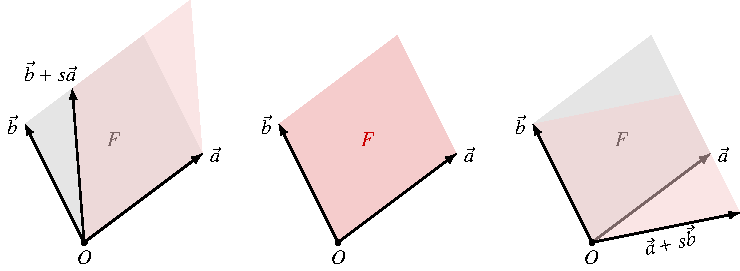
\includegraphics{chapters/040-green/images/parallelogramm.pdf}
\caption{Die Parallelogrammfläche ist eine bilineare Funktion der
Kantenvektoren.
Die Parallelogrammfläche ändert nicht, wenn man einen Kantenvektor
um ein Vielfaches des anderen ändert.
Dies ist die gemeinsame Eigenschaft vieler physikalischer Eigenschaften,
die oft mit dem Vektorprodukt modelliert werden.
\label{buch:green:2vektoren:fig:parallelogramm}}
\end{figure}

Zwei Vektoren $\vec{a}$ und $\vec{b}$ spannen eine Parallelogramm auf.
Der Flächeninhalt ändert sich nicht, wenn man die Spitze des Vektors
$\vec{a}$ parallel zur Richtung von $\vec{b}$ verschiebt.
Er ändert sich auch nicht, wenn man die Spitze von $\vec{b}$ parallel
zur Richtung von $\vec{a}$ verschiebt.

Das Vektorprodukt hat die passenden Eigenschaften.
Ändert man den Vektor $\vec{a}$ in $\vec{a}+t\vec{b}$, ändert sich das
Vektorprodukt
\begin{equation}
(\vec{a}+t\vec{b})\times\vec{b}
=
\vec{a}\times\vec{b} + t(\underbrace{\vec{b}\times\vec{b}}_{\displaystyle=0})
=
\vec{a}\times\vec{b}
\label{buch:green:2vektoren:eqn:parallelogramm1}
\end{equation}
nicht.
Ebenso ändert sich das Vektorprodukt nicht, wenn man $\vec{b}$ durch
$\vec{b}+s\vec{a}$ ersetzt, denn
\begin{equation}
\vec{a}\times(\vec{b}+s\vec{a})
=
\vec{a}\times\vec{b}
+
s(\underbrace{\vec{a}\times\vec{a}}_{\displaystyle=0})
=
\vec{a}\times\vec{b}.
\label{buch:green:2vektoren:eqn:parallelogramm2}
\end{equation}
Für Vektoren im dreidimensionalen Raum ist das Vektorprodukt ein 
Realisierung der einleitend formulierten Eigenschaften.
Die Eigenschaft ist aber auch korrekt in zwei Dimensionen, wo es
das Vektorprodukt nicht gibt.

Der Flächeninhalt eines Parallelogramms ist ausser in zwei Dimensionen
nicht nur eine Zahl, die Lage des Parallelgramms gehört genauso zur
vollständigen Beschreibung der Parallelogrammfläche.
Das Vektorprodukt in drei Dimensionen trägt dem Rechnung, indem
es als Normale auf dem Parallelgramm die Orientierung im dreidimensionalen
Raum festlegt.
In einem höherdimensionalen Raum reicht jedoch ein einzelner auf
einem Parallelogramm orthogonaler Vektor nicht aus, um die Lage im
Raum vollständig festzulegen.

Eine Parallelogrammfläche wird also beschrieben durch ein neues
mathematisches Objekt, welches mit einer bilinearen Operation aus
zwei Vektoren $\vec{a}$ und $\vec{b}$ gebildet wird.
Wir bezeichnen es provisorisch als den 2-Vektor $\vec{a}\wedge\vec{b}$.
Das Zeichen $\wedge$ funktioniert wie ein Produkt, es ist eine 
bilineare Operation zwischen Vektoren mit den Rechenregeln
\begin{align}
(\vec{a}_1+\vec{a}_2)\wedge\vec{b}
&=
\vec{a}_1\wedge\vec{b}+\vec{a}_2\wedge\vec{b}
\notag
\\
\vec{a}\wedge(\vec{b}_1+\vec{b}_2)
&=
\vec{a}\wedge\vec{b}_1 + \vec{a}\wedge\vec{b}_2
\notag
\\
(\lambda\vec{a})\wedge\vec{b}
&=
\lambda(\vec{a}\wedge\vec{b})=\vec{a}\wedge(\lambda\vec{b})
\notag
\\
\vec{a}\wedge\vec{a}&=0.
\label{buch:green:2vektoren:eqn:aa0}
\end{align}
Die ersten drei Regeln drücken aus, dass der 2-Vektor $\vec{a}\wedge\vec{b}$
bilinear ist oder gleichbedeutend, dass das Wedge-Produkt das
Distributivgesetz erfüllt.
Die letzte Regel genügt, um die zu
\eqref{buch:green:2vektoren:eqn:parallelogramm1}
und
\eqref{buch:green:2vektoren:eqn:parallelogramm2}
äquivalenten Regeln
\begin{equation}
\begin{aligned}
\vec{a}\wedge(\vec{b}+t\vec{a})
&=
\vec{a}\wedge\vec{b}
\qquad \forall t\in\mathbb{R}
\\
(\vec{a}+s\vec{b})\wedge\vec{b}
&=
\vec{a}\wedge\vec{b}
\qquad \forall s\in\mathbb{R}
\end{aligned}
\label{buch:green:2vektoren:eqn:grundeigenschaft}
\end{equation}
für das Wedge-Produkt sicherzustellen.
Aus \eqref{buch:green:2vektoren:eqn:aa0} lässt sich aber auch
ableiten, dass für beliebige Vektoren $\vec{a}$ und $\vec{b}$
\begin{align*}
0
&=
(\vec{a}+\vec{b})\wedge(\vec{a}+\vec{b})
\\
&=
\underbrace{\vec{a}\wedge\vec{a}}_{\displaystyle=0}
+
\vec{a}\wedge\vec{b}
+
\vec{b}\wedge\vec{a}
+
\underbrace{\vec{b}\wedge\vec{b}}_{\displaystyle=0}
\\
\Rightarrow\qquad
\vec{a}\wedge\vec{b}
&=
-\vec{b}\wedge\vec{a}
\end{align*}
gilt, das Wedge-Produkt ist also notwendigerweise antikommutativ.

%
% Drehmoment und Drehimpuls
%
\subsubsection{Drehmoment und Drehimpuls}
Eine Kraft $\vec{F}$, die auf einen im Nullpunkt drehbar gelagerten
starren Körper wirkt, versucht diesen Körper in Drehung zu versetzen.
Der Angriffspunkt $P$ der Kraft habe den Ortsvekor $\vec{r}$.
Je grösser die Kraft $\vec{F}$ oder je länger der Vektor $\vec{r}$,
desto grösser wird auch die Drehwirkung sein.
Wir haben also wieder mit einer physikalischen Grösse zu tun, die
bilinear von zwei Vektoren abhängt.

Ändert man die Kraft, indem man eine Komponente parallel zu $\vec{r}$
hinzufügt, dann ändert sich die Auswirkung auf den Drehzustand des
Körpers nicht.
Sie ändert sich auch nicht, wenn man den Ansatzpunkt der Kraft
auf einer Geraden durch den Punkt $P$ mit Richtung $\vec{F}$
verschiebt.
In der Physik wird dies oft dadurch ausgedrückt, dass die Kraft
ein linienflüchtiger Vektor sei.
Diese Eigenschaften decken sich wieder mit den Regeln
\eqref{buch:green:2vektoren:eqn:grundeigenschaft}
des Wedge-Produktes.

In der Physik wird das Drehmoment meistens als Vektorprodukt
$\vec{M}=\vec{r}\times\vec{F}$ modelliert.
Die Überlegungen des vorangegangenen Abschnitts zeigen, dass
es genausogut oder sogar besser durch den 2-Vektor
$\vec{r}\wedge\vec{F}$ beschrieben werden kann.

Beim Drehimpuls wird die Unzulänglichkeit des einfachen, auf
dem Vektorprodukt basierenden Modells offensichtlich.
Versucht man die Drehung durch einen Vektor $\vec{\omega}$ zu
beschreiben, der die Richtung der Drehachse und die Winkelgeschwindigkeit
als Länge enthält, dann ist der Drehimpuls nicht notwendigerweise
parallel zur Richtung der Drehachse.
Vielmehr gibt es eine lineare Abbildung, die den Drehimpulsvektor
$\vec{L}$ aus $\vec{omega}$ berechnet.
Man darf erwarten, dass die Verwirrung aufgelöst wird, wenn man
Drehmoment und Drehimpuls als 2-Vektoren modelliert und den Zusammenhang
dazwischen durch einen Tensor erklärt.

%
% Lorentz-Kraft
%
\subsubsection{Lorentz-Kraft}
%
% fig-lorentz.tex
%
% (c) 2025 Prof Dr Andreas Müller
%
\begin{figure}
\centering
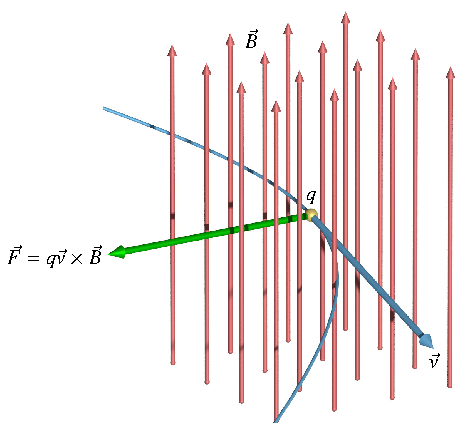
\includegraphics{chapters/040-green/images/lorentz.pdf}
\caption{Die Lorentz-Kraft auf eine bewegte Ladung hängt bilinear
von der Geschwindigkeit $\vec{v}$ und vom magnetischen Induktionsfeld
$\vec{B}$ ab.
Sie hat die Eigenschaften eines 2-Vektors.
\label{buch:green:2vektoren:fig:lorentz}}
\end{figure}

Die Lorentz-Kraft ist die Kraft, die eine bewegte Ladung in einem
magnetischen Feld erfährt.
Sie ist proportional zur Geschwindigkeit, eine ruhende Ladung
wird von einem Magnetfeld nicht beeinflusst.
Sie ist auch proportional zur Stärke des magnetischen Feldes.
Die Lorentz-Kraft ist also eine bilineare Funktion der
Geschwindigkeit $\vec{v}$ der Ladung und des magnetischen
Induktionsfeldes $\vec{B}$

Die Lorentz-Kraft verschwindet, falls sich die Ladung parallel zur
magnetischen Feldrichtung bewegt.
Insbesondere ändert sie auch nicht, wenn die Geschwindigkeit der
Ladung um eine Komponenten parallel zu $\vec{B}$ verändert wird.
Umgekehrt ändert die Lorentz-Kraft auch nicht, wenn dem Feld
eine Komponenten parallel zur Geschwindigkeit der Ladung hinzugefügt
wird.
Auch die Lorentz-Kraft erfüllt also die grundlegenden
Rechenregeln \eqref{buch:green:2vektoren:eqn:grundeigenschaft}.
In der Physik wird sie daher meistens als das Vektorprodukt
\[
\vec{F}_L
=
q\vec{v}\times \vec{B}
\]
beschrieben, worin $q$ die Ladung ist.
Nach den früheren Überlegungen ist sie aber eher als ein weiteres
Beispiel eines 2-Vektors anzusehen.

Es wird sich später zeigen, dass die Elektrodynamik besser in einer
vierdimensionalen Raumzeit beschrieben wird, die auch die Basis für
die spezielle und allgemeine Relatiitätstheorie ist.
Die Identifikation von 2-Vektoren mit Vektoren ist darin nicht
mehr möglich.
Die Verwendung von 2-Vektoren wird aber ermöglichen, die elektrische 
und die Lorentz-Kraft auf einheitliche Art zu beschreiben.

%
% Basis, Wedge-Produkt, Rechenregeln
%
\subsection{Der Vektorraum der 2-Vektoren}
Die 2-Vektoren sind also eine neue Art von Vektoren, die aus den
gewöhnlichen Vektoren in $\mathbb{R}^n$ gebildet werden können.
Sie bilden selbst wieder einen Vektorraum, da man sie addieren
und mit reellen Zahlen multiplizieren kann.
In gewissen Fällen, zum Beispiel im dreidimensionalen Raum, kann
man für 2-Vektoren wieder eine anschauliche Darstellung ähnlich den
Pfeilen für Vektoren finden.
Es wurde aber bereits darauf hingewiesen, dass die eigentlich nicht
zulässig ist, da weder die Dimensionen noch die Symmetrieeigenschaften
vergleichbar sind.
Wenn zwei Vektoren geometrische Längen beschreiben, dann haben sie
die Längeneinheit als Masseinheit.
Ihr Wedge-Produkt muss dann die Flächeneinheit als Masseinheit haben,
kann also nicht im gleichen Raum dargestellt werden.

\subsubsection{Basis}
Ausgehend von der Basis $\vec{e}_1,\dots,\vec{e}_n$ lassen sich jetzt
alle Wedge-Produkte
\[
\vec{e}_i\wedge \vec{e}_k
\]
mit $i\ne k$ bilden.
Wegen
\[
\vec{e}_i\wedge\vec{e}_k
=-
\vec{e}_k\wedge\vec{e}_i
\]
können wir auf die Produkte $\vec{e}_i\wedge\vec{e}_k$ mit $i<k$
beschränken, die wir alle als linear unabhängig annehmen müssen.

\begin{definition}[Raum der 2-Vektoren]
Sei $V$ ein $n$-dimensioinaler reeller Vektorraum, dann ist die Menge
\[
{\textstyle
\bigwedge^2 V}
= \langle \vec{a}\wedge\vec{b} \mid \vec{a},\vec{b}\in V \rangle
\]
ein $n(n-1)/2$-dimensionaler reeller Vektorraum.
Bilden $b_1,\dots,b_n\in V$  eine Basis von $V$, dann bilden die Vektoren
\[
b_i\wedge b_k,\qquad i<k
\]
eine Basis von $\bigwedge^2 V$.
\end{definition}

In einem zweidimensionalen Raum $\mathbb{R}^2$ gibt es nur einen
einzigen 2-Vektor $\vec{e}_1\wedge\vec{e}_2$, nur schon aus diesem
Grund ist es nicht möglich, einen 2-Vektor als Vektor in $\mathbb{R}^2$
darzustellen.

In einem dreidimensionalen Raum $\mathbb{R}^3$ gibt es die drei
Basisvektoren
\[
\vec{e}_1\wedge\vec{e}_2,\quad
\vec{e}_1\wedge\vec{e}_3
\quad\text{und}\quad
\vec{e}_2\wedge\vec{e}_3.
\]
Tatsächlich lässt sich auch eine Abbildung der 2-Vektoren auf
die Vektoren finden, die das Wedge-Produkt auf das Vektorprodukt
abbildet.
Sie wird aus der Komponentenformel weiter unten abgeleitet.

In einem vierdimensionalen Raum $\mathbb{R}^4$ gibt es die sechs
linear unabhängigen Basisvektoren
\[
\vec{e}_1\wedge\vec{e}_2,\quad
\vec{e}_1\wedge\vec{e}_3,\quad
\vec{e}_1\wedge\vec{e}_4,\quad
\vec{e}_2\wedge\vec{e}_3,\quad
\vec{e}_2\wedge\vec{e}_4,
\quad\text{und}\quad
\vec{e}_3\wedge\vec{e}_4.
\]
Da der Raum der 2-Vektoren mehr Dimensionen als der Raum 
der Vektoren hat, ist es grundsätzlich unmöglich, die 2-Vektoren
durch Vektoren zu visualisieren.

\subsubsection{Komponentenformel}
In der Basis $\vec{e}_1,\dots,\vec{e}_n$ kann jeder Vektor als
Linearkombination
\[
\vec{a}
=
a^1\vec{e}_1+\dots+a^n\vec{e}_n
=
\sum_{i=1}^n a^i\vec{e}_i
\qquad\text{und}\qquad
\vec{b}
=
b^1\vec{e}_1+\dots+b^n\vec{e}_n
\sum_{k=1}^n b^k\vec{e}_k
\]
geschrieben werden.
Das Wedge-Produkt der beiden Vektoren ist
\begin{align}
\vec{a}\wedge\vec{b}
&=
\biggl(
\sum_{i=1}^n a^i\vec{e}_i
\biggr)
\wedge
\biggl(
\sum_{k=1}^n b^k\vec{e}_k
\biggr)
\notag
\\
&=
\sum_{i,k=1}^n a^ib^k\,\vec{e}_i\wedge\vec{e}_k
\notag
\intertext{Die Wedge-Produkt $\vec{e}_i\wedge\vec{e}_i=0$ verschwinden,
es bleibt daher nur}
&=
\sum_{i\ne k} a^ib^k \, \vec{e}_i\wedge\vec{e}_k.
\notag
\intertext{Als Basis werden aber nur die Produkte mit $i<k$ verwendet,
wir zerlegen die Summe daher in die Fälle $i<k$ und $k<i$:}
&=
\sum_{i < k} a^ib^k \, \vec{e}_i\wedge\vec{e}_k
+
\sum_{i > k} a^ib^k \, \vec{e}_i\wedge\vec{e}_k
\notag
\\
&=
\sum_{i < k} a^ib^k \, \vec{e}_i\wedge\vec{e}_k
-
\sum_{i > k} a^ib^k \, \vec{e}_k\wedge\vec{e}_i.
\notag
\intertext{In der zweiten Summe ist der erste Index jetzt wieder kleiner
als der zweite, wir können in dieser Summe die Indizes umbennennen
und erhalten}
&=
\sum_{i < k} a^ib^k \, \vec{e}_i\wedge\vec{e}_k
-
\sum_{k > i} a^kb^i \, \vec{e}_i\wedge\vec{e}_k.
\notag
\intertext{Damit können die beiden Summen wieder in eine einzige
zusammengefasst werden.
Daraus lassen sich die Komponenten von}
\vec{a}\wedge\vec{b}
&=
\sum_{i<k} (a^ib^k-a^kb^i)\,\vec{e}_i\wedge\vec{e}_k
\label{buch:green:2vektoren:eqn:komponentenformel}
\end{align}
in der Basis der 2-Vektoren $\vec{e}_i\wedge\vec{e}_k$ ausdrücken.

\subsubsection{Komponentenformel und Vektorprodukt}
Das Vektorprodukt wird in Komponenten als
\[
\begin{pmatrix} a^1 \\ a^2 \\ a^3 \end{pmatrix}
\times
\begin{pmatrix} b^1 \\ b^2 \\ b^3 \end{pmatrix}
=
\begin{pmatrix} a^2b^3-a^3b^2 \\ a^3b^1-a^1b^3 \\ a^1b^2-a^2b^1 \end{pmatrix}
\]
definiert.
Die Komponenten des Vektorprodukts sehen der allgemeinen
Komponentenformel~\eqref{buch:green:2vektoren:eqn:komponentenformel}
des Wedge-Produktes sehr ähnlich.
Tatsächlich kann man den Zusammenhang noch etwas offensichtlicher
machen, indem man die lineare Abbildung $f:\bigwedge^2V\to V$
verwendet, die auf den Basisvektoren durch
\[
\vec{e}_1\wedge\vec{e}_2 \mapsto \vec{e}_3
\vec{e}_1\wedge\vec{e}_3 \mapsto -\vec{e}_2
\vec{e}_2\wedge\vec{e}_3 \mapsto \vec{e}_1
\]
definiert sind.
Aus dem 2-Vektor $\vec{a}\wedge\vec{b}$ wird dadurch
\begin{align*}
f(\vec{a}\wedge\vec{b})
&=
f\bigl((a^1b^2-a^2b^1)\vec{e}_1\wedge\vec{e}_2
      +(a^1b^3-a^3b^1)\vec{e}_1\wedge\vec{e}_3
      +(a^2b^3-a^3b^2)\vec{e}_2\wedge\vec{e}_3\bigr)
\\
&=
(a^1b^2-a^2b^1)\,f(\vec{e}_1\wedge\vec{e}_2)
+(a^1b^3-a^3b^1)\,f(\vec{e}_1\wedge\vec{e}_3)
+(a^2b^3-a^3b^2)\,f(\vec{e}_2\wedge\vec{e}_3)
\\
&=
(a^1b^2-a^2b^1) \vec{e}_3
+(a^1b^3-a^3b^1) (-\vec{e}_2)
+(a^2b^3-a^3b^2) \vec{e}_1
\\
&=
(a^2b^3-a^3b^2) \vec{e}_1
+(a^3b^1-a^1b^3) \vec{e}_2
+(a^1b^2-a^2b^1) \vec{e}_3
\\
&=
\vec{a}\times\vec{b}.
\end{align*}
In diesem Lichte kann man das Vektorprodukt als ein spezielle Darstellung
des Wedge-Produktes durch Vektoren statt 2-Vektoren ansehen, die allerdings
nur in drei Dimensionen möglich ist.

%
% Alternative Darstellungen des Wedge-Produktes
%
\subsection{Alternative Darstellungen des Wedge-Produktes}
Die algebraischen Eigenschaften der 2-Vektoren und des Wedge-Produktes
wurden aus geometrischen oder physikalischen Prinzipien hergeleitet.
Angesichts der Vielfalt der mathematischen Werkzeuge, die zur Beschreibung
der physikalischen Realität zur Verfügung stehen, erwartet man daher,
dass die algebraische Struktur sich in verschiedenen mathematischen
Konstrukten wiederfinden lässt.

\subsubsection{Das Vektorprodukt als Kommutator von Matrizen}
Wir betrachten die Menge 
\[
V
=
\{ A\in M_3(\mathbb{R}) \mid A^t=-A\}
\]
der antisymmetrischen $3\times 3$-Matrizen.
Solche Matrizen sind von der Form
\begin{equation}
A
=
\begin{pmatrix}
  0  &  a_3 & -a_2 \\
-a_3 &   0  &  a_1 \\
 a_2 & -a_1 &   0
\end{pmatrix}.
\label{buch:green:2vektoren:eqn:antisym}
\end{equation}
Der {\em Kommutator} zweier Matrizen ist $[A,B]=AB-BA$ und ergibt
für Matrizen der Form~\eqref{buch:green:2vektoren:eqn:antisym}
\begin{align*}
AB
&=
\begin{pmatrix}
  0  &  a_3 & -a_2 \\
-a_3 &   0  &  a_1 \\
 a_2 & -a_1 &   0
\end{pmatrix}
\begin{pmatrix}
  0  &  b_3 & -b_2 \\
-b_3 &   0  &  b_1 \\
 b_2 & -b_1 &   0
\end{pmatrix}
\\
&=
\begin{pmatrix}
-a_2b_2-a_3b_3 &     a_2b_1     & a_3b_1         \\
 a_1b_2        & a_1b_1+a_3b_3  & a_3b_2         \\
 a_1b_3        &     a_2b_3     & -a_1b_1-a_2b_2 
\end{pmatrix}
\\
BA
&=
\begin{pmatrix}
  0  &  b_3 & -b_2 \\
-b_3 &   0  &  b_1 \\
 b_2 & -b_1 &   0
\end{pmatrix}
\begin{pmatrix}
  0  &  a_3 & -a_2 \\
-a_3 &   0  &  a_1 \\
 a_2 & -a_1 &   0
\end{pmatrix}
\\
&=
\begin{pmatrix}
-a_2b_2-a_3b_3  &      a_1b_2    &    a_1b_3     \\
     a_2b_1     & -a_1b_1-a_3b_3 &    a_2b_3     \\
     a_3b_1     &      a_3b_2    & -a_1b_1-a_2b_2
\end{pmatrix}
\\
[A,B]
&=
AB-BA
=
\begin{pmatrix}
        0        &   a_2b_1-a_1b_2  & -(-a_3b_1+a_1b_3) \\
-(a_2b_1-a_1b_2) &         0        &    a_3b_2-a_2b_3  \\
  a_1b_3-a_3b_1  & -(a_3b_2-a_2b_3) &          0
\end{pmatrix}.
\end{align*}
Diese Matrix ist wieder von der Form 
\eqref{buch:green:2vektoren:eqn:antisym}
und die Einträge sind die Komponenten des Vektorproduktes.
Das Vektorprodukt lässt sich also durch den Matrixkommutator
auf der Menge darstellen.

\subsubsection{Die Lie-Algebra einer Matrizengruppe}
TODO XXX


%
% 2-Formen
%
\section{Tensoren zweiter Stufe, 2-Vektoren und 2-Formen auf Mannigfaltigkeiten
\label{buch:green:section:2formen}}
\kopfrechts{2-Formen}
Die Algebra der 2-Vektoren ist nicht auf einen Vektorraum beschränkt,
sie kann auch auf die Tangentialvektoren einer $n$-dimensionalen
Mannigfaltigkeit angewendet werden.
Ein 2-Vektor auf einer Mannigfaltigkeit ist dann ein Tensor zweiter
Stufe vom Typ $(2,0)$.
In einer Karte wird er gegeben durch eine Grösse $a^{ik}$ mit zwei
kontravarianten Indizes.
Gegenüber einem beliebigen Tensor zweiter Stufe zeichnet sich der 
2-Vektor dadurch aus, dass $a^{ik}$ antisymmetrisch ist, dass also
$a^{ik}=-a^{ki}$ gilt.

%
% Notation für Tensoren
%
\subsection{Notation für Tensoren}
In Kapitel~\ref{chapter:kurvenintegral} haben wir zwar den Begriff des
Tensors eingeführt, aber nur eine Notation für Vektoren eingeführt.
Wenn mit Tensoren gerechnet worden ist, kam immer nur die Komponenten
in einer Karte zur Anwendung.
Das Wedge-Produkt von Vektoren hat 2-Vektoren ergeben, kann aber
nicht alle Tensoren zweiter Stufe darstellen.
Wir erweitern daher die Notation, indem wir wie bei der Einführung der
Basis für die 2-Vektoren, neue Basisvektoren für die Tensoren wie 
folgt definieren.

\begin{definition}
\label{buch:green:tensoren:definition:tensorprodukt}
Sei $V$ ein $n$-dimensionaler reeller Vektorraum mit Basis
$\vec{e}_1,\dots,\vec{e}_n$.
Der Vektorraum
\[
V^{\otimes p}
=
\underbrace{
V\otimes\dots\otimes V
}_{\displaystyle \text{$p$ Faktoren}}
=
\langle \vec{e}_{i_1}\otimes\dots\otimes \vec{e}_{i_p}
\mid
1\le 
i_1,\dots,i_p
\le n
\rangle
\]
heisst das $p$-fache Tensorprodukt von $V$.
\index{Tensorprodukt}%
Ein Tensor $p$-ter Stufe ist also von der Form
\[
a_{i_1\dots i_p}\vec{e}_{i_1}\otimes\dots\otimes\vec{e}_{i_p}
\]
mit Koeffizienten $a_{i_1\dots i_p}\in\mathbb{R}$.
\end{definition}

Ein 2-Vektor ist ein Tensor in $V^{\otimes 2}$, der antisymmetrisch ist.
Für die Basisvektoren der 2-Vektoren können daher als Tensoren
\[
\vec{e}_i\wedge\vec{e}_k
=
\vec{e}_i\otimes\vec{e}_k
-
\vec{e}_k\otimes\vec{e}_i
\]
geschrieben werden.
Ein 2-Vektor ist also allgemein eine Linearkombination
\begin{equation}
a^{ik}\vec{e}_i\otimes\vec{e}_k
\label{buch:green:tensoren:eqn:2tensor}
\end{equation}
mit $a^{ik}=-a^{ki}$.

Die Definition~\ref{buch:green:tensoren:definition:tensorprodukt}
berücksichtigt die Transformationseigenschaften nicht,
die die Komponenten eines aus Tangentialvektoren gebildeten
Tensors zusätzlich erfüllen müssen.
Ein kontravarianter Tensor zweiter Stufe kann dann als
\[
a
=
a^{ik}(x) \frac{\partial}{\partial x^i}\otimes\frac{\partial}{\partial x^k}
\]
geschrieben werden, wobei die bei einem Koordinatenwechsel die
Indizes $i$ und $k$ kontravariant transformiert werden.
Ein 2-Vektor auf der Mannigfaltigkeit entsteht dann aus den Koeffizienten
$a^{ik}(x)$ durch
\[
\sum_{i<k}
a^{ik}
\frac{\partial}{\partial x^i}
\wedge
\frac{\partial}{\partial x^k}
=
a^{ik}(x)
\frac{\partial}{\partial x^i}
\otimes
\frac{\partial}{\partial x^k},
\]
wobei $a^{ik}(x)=-a^{ki}(x)$ sein muss.

%
% 2-Formen
%
\subsection{2-Formen}
Linearformen sind lineare Abbildungen von Vektoren auf reelle Zahlen.
Linearformen können aber auch auf Tensoren zweiter Stufe definiert werden.
Eine Linearform $f\colon V^{\otimes 2}\to\mathbb{R}$ muss den Basisvektoren
$\vec{e}_i\otimes\vec{e}_k$ einen Wert zuordnen.
Schreiben wir $f(\vec{e}_i\otimes\vec{e}_k)=f_{ik}$, dann ist der Wert
auf einem Tensor der Form
\eqref{buch:green:tensoren:eqn:2tensor}
gegeben durch
\[
f\bigl(
a^{ik}\vec{e}_i\otimes \vec{e}_k
\bigr)
=
a^{ik}
f_{ik}.
\]
Eine Linearform auf $V^{\otimes 2}$ kann auch aus zwei Linearformen
$f$ und $g$ auf $V$ konstruiert werden.
Solche Linearformen können durch die Werte
\[
f_i = f(\vec{e}_i) 
\qquad\text{und}\qquad
g_k = f(\vec{e}_k)
\]
auf den Basisvektoren konstruiert werden.
Auf dem Tensor $a$ ergibt sie den Wert
\[
(f\otimes g)
=
a^{ik}f(\vec{e}_i)g(\vec{e}_k)
=
a^{ik}f_ig_k.
\]


%
% Flächenintegrale
%
\section{Flächenintegrale von 2-Formen
\label{buch:green:section:integral}}
\kopfrechts{Flächenintegrale}
In Abschnitt~\ref{buch:kurvenintegral:section:1form} wurde gezeigt,
wie das Integral einer 1-Form entlang einer Kurve auf
koordinatensystemunabhängige Grösse definiert werden kann.
Entscheidend war die Erkenntnis, dass das Integral der Werte einer
Funktion entlang der Kurve von der Parametrisierung, also dem
Koordinatensystem, der Kurve abhängt.
Nur eine 1-Form hat das richtige Transformationsverhalten beim
Wechsel des Koordinatensystems, das zu einer koordinatensystemunabhängigen
Definition führt.
In diesem Abschnitt wird diese Überlegung auf zweifache Integrale
verallgemeinert.

%
% Integral einer 2-Form auf R^2
%
\subsection{Integral einer 2-Form auf $\mathbb{R}^2$}
Wir betrachten eine differenzierbare Funktion
$f\colon \mathbb{R}^2\to\mathbb{R}$ zweier Variablen.
Zusätzlich sei angenommen, dass $f$ kompakten Träger hat. 
Dann ist dass Integral von $f$ über $\mathbb{R}^2$ wohldefiniert
und kann mit Hilfe des Satzes von Fubini als iteriertes Integral
\index{Satz!von Fubini}%
\begin{equation}
\int_{\mathbb{R}^2} f(x^1,x^2)\,dx^1\,dx^2
=
\int_{\mathbb{R}} \biggl(\int_{\mathbb{R}} f(x^1,x^2) \,dx^1\biggr) \,dx^2
=
\int_{\mathbb{R}} \biggl(\int_{\mathbb{R}} f(x^1,x^2) \,dx^2\biggr) \,dx^1
\label{buch:green:flaechenintegral:eqn:int2}
\end{equation}
berechnet werden.
Die Klammern sind nur zur Verdeutlichung.
Das innere Integral hängt von einem Parameter $x^2$ bzw.~$x^1$ ab.
Das Resultat der Integration ist daher nur noch eine differenzierbare
Funktion von $x^2$ bzw.~$x^1$, die wieder integrierbar ist.

Das Integral~\eqref{buch:green:flaechenintegral:eqn:int2} kann jedoch
nicht koordinatenunabhängig sein.
%
% fig-volint.tex
%
% (c) 2025 Prof Dr Andreas Müller
%
\begin{figure}
\centering
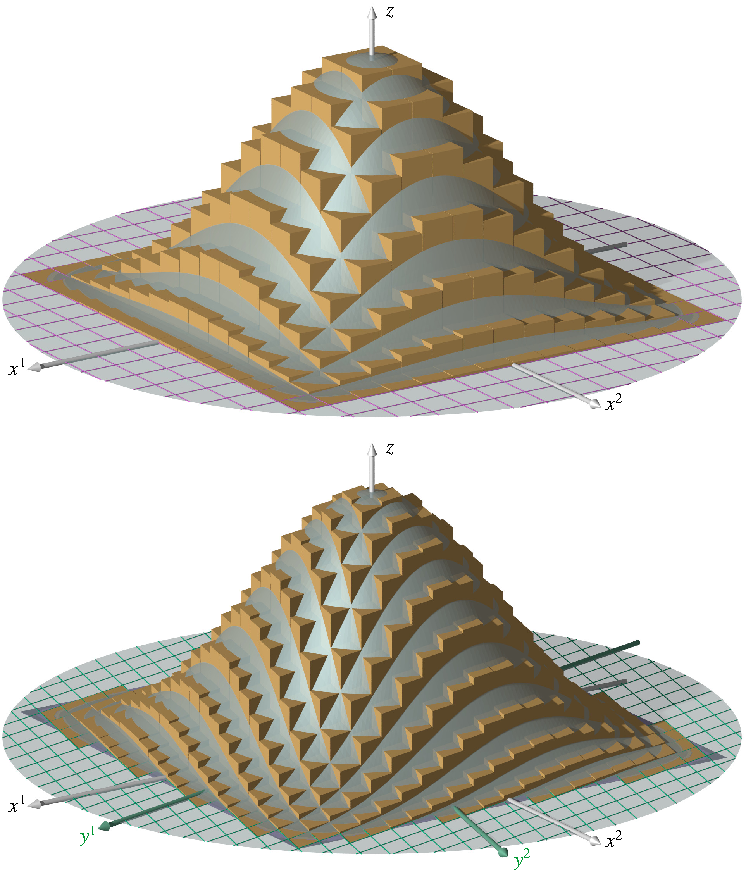
\includegraphics[width=\textwidth]{chapters/040-green/images/volint.pdf}
\caption{Volumen unter dem Graphen der Funktion $f(x^1,x^2)$ berechnet mit
zwei verschiedenen Parametrisierungen der Ebene.
In den $(x^1,x^2)$-Koordinaten wird das Volumen als Summe von Quadern
approximiert.
In den $(y^1,y^2)$-Koordinaten werden Prismen mit parallelogrammförmigen
Grundflächen aufaddiert.
Eine koordinatenunabhängige Grösse entsteht nur, wenn die Änderung
der Prismengrundfläche berücksichtigt wird.
\label{buch:green:fig:volint}}
\end{figure}
%
Dazu interpretieren wir das Integral als das Volumen unter einer der 
Fläche, die der Graph der Funkion $f(x^1,x^2)$ ist.
Es setzt sich approximativ zusammen aus kleinen Quadern mit
rechteckiger Grundfläche $\Delta x^1 \times \Delta x^2$ und Höhe
$f(x^1,x^2)$.
Das gleiche Volumen wird nach einer lineare Transformation 
\[
\begin{aligned}
x^1 &= a^1\mathstrut_1 y^1 + a^1\mathstrut_2 y^2 \\
x^2 &= a^2\mathstrut_1 y^1 + a^2\mathstrut_2 y^2 
\end{aligned}
\]
durch eine Summe von Prismen approximiert, die Höhe $f(y^1,y^2)$ haben,
\index{Prisma}%
aber als Grundfläche ein Parallelogramm, mit den Kantenvektoren
\[
\begin{pmatrix}
a^1\mathstrut_1\\
a^2\mathstrut_1
\end{pmatrix}
\Delta y^1
\qquad\text{und}\qquad
\begin{pmatrix}
a^1\mathstrut_2\\
a^2\mathstrut_2
\end{pmatrix}
\Delta y^2.
\]
Der Flächeneinhalt eines solchen Parallelogramms ist die Determinante
\[
F
=
\left|
\begin{matrix}
a^1\mathstrut_1 & a^1\mathstrut_2 \\
a^2\mathstrut_1 & a^2\mathstrut_2
\end{matrix}
\right|
\Delta y^1\cdot \Delta y^2.
\]
Um also das gleiche Volumen wie von
\eqref{buch:green:flaechenintegral:eqn:int2}
zu erhalten, muss das Integral
\[
\int_{\mathbb{R}^2}
f(x^1,x^2)
\,dx^1\,dx^2
=
\int_{\mathbb{R}^2}
f(y^1,y^2)
\left|
\begin{matrix}
a^1\mathstrut_1 & a^1\mathstrut_2 \\
a^2\mathstrut_1 & a^2\mathstrut_2
\end{matrix}
\right|
\,dy^1\,dy^2
\]
berechnet werden.
Die Verzerrung des Gitters ist in Abbildung~\ref{buch:green:fig:volint}
dargestellt.
Der Determinantenfaktor rechnet das Volumen des Einheitsquadrates in den
$(y^1,y^2)$-Koordinaten um in den Flächeninhalt des Grundseitenparallelogramms
eines Prismas in den $(x^1,x^2)$-Koordinaten.

Eine Funktion hat also nicht die richtigen Transformationseigenschaften.
Die Determinante
\[
\det A
=
a^1\mathstrut_1
a^2\mathstrut_2
-
a^1\mathstrut_2
a^2\mathstrut_1
\]
bedeutet, dass bei der Transformation immer zwei Faktoren aus der
Transformationsmatrix auftauchen, dies ist nicht möglich bei einem
Tensor erster Stufe.
Nur mit einem Tensor zweiter Stufe ist es möglich, solche Produkte 
in der Transformationsformel zu haben.

Seien also jetzt $f_{ik}$ die Koeffizienten eines Tensors 
zweiter Stufe in $x$-Koordinaten und $\tilde{f}_{lm}$ die Koeffizienten
des Tensors in den $y$-Koordinaten.
Die Transformationsformel ist dann
\begin{align}
\tilde{f}_{lm}
&=
\sum_{i,k=1}^2
f_{ik}\, a^i\mathstrut_l\, a^k\mathstrut_m.
\intertext{Die Transformation soll nur die Determinante von $A$
hinzufügen.
Schreibt man die Transformationsformeln aus, erhält man}
\tilde{f}_{11}
&=
f_{11}\, a^1\mathstrut_1\, a^1\mathstrut_1
+
f_{12}\, a^1\mathstrut_1\, a^2\mathstrut_1
+
f_{21}\, a^2\mathstrut_1\, a^1\mathstrut_1
+
f_{22}\, a^2\mathstrut_1\, a^2\mathstrut_1
\\
\tilde{f}_{12}
&=
f_{11}\, a^1\mathstrut_1\, a^1\mathstrut_2
+
f_{12}\, a^1\mathstrut_1\, a^2\mathstrut_2
+
f_{21}\, a^2\mathstrut_1\, a^1\mathstrut_2
+
f_{22}\, a^2\mathstrut_1\, a^2\mathstrut_2
\\
\tilde{f}_{21}
&=
f_{11}\, a^1\mathstrut_2\, a^1\mathstrut_1
+
f_{12}\, a^1\mathstrut_2\, a^2\mathstrut_1
+
f_{21}\, a^2\mathstrut_2\, a^1\mathstrut_1
+
f_{22}\, a^2\mathstrut_2\, a^2\mathstrut_1
\\
\tilde{f}_{22}
&=
f_{11}\, a^1\mathstrut_2\, a^1\mathstrut_2
+
f_{12}\, a^1\mathstrut_2\, a^2\mathstrut_2
+
f_{21}\, a^2\mathstrut_2\, a^1\mathstrut_2
+
f_{22}\, a^2\mathstrut_2\, a^2\mathstrut_2.
\end{align}
Diese Formeln können nur dann nur einen Faktor $\det A$ ergeben,
wenn alle Terme, in denen Produkt von $a^s\mathstrut_r$ wie in der
Determinante vorkommen.
Daraus kann man schliessen, dass $f_{11}=f_{12}=0$ sein muss.
Es bleiben  dann die Gleichungen
\begin{align*}
0
&=
f_{12}\, a^1\mathstrut_1\, a^2\mathstrut_1
+
f_{21}\, a^2\mathstrut_1\, a^1\mathstrut_1
=
(f_{12}+f_{21})\, a^1\mathstrut_1\, a^2\mathstrut_1
\\
\tilde{f}_{12}
&=
f_{12}\, a^1\mathstrut_1\, a^2\mathstrut_2
+
f_{21}\, a^2\mathstrut_1\, a^1\mathstrut_2
\\
\tilde{f}_{21}
&=
f_{12}\, a^1\mathstrut_2\, a^2\mathstrut_1
+
f_{21}\, a^2\mathstrut_2\, a^1\mathstrut_1
\\
0
&=
f_{12}\, a^1\mathstrut_2\, a^2\mathstrut_2
+
f_{21}\, a^2\mathstrut_2\, a^1\mathstrut_2
=
(f_{12}+f_{21}) a^1\mathstrut_2\, a^2\mathstrut_2
\end{align*}
Die erste und die letzte dieser Gleichungen können nur erfüllt sein,
wenn $f_{12}=-f_{21}$, $f$ muss also ein antisymmetrischer
Tensor sein.
Es bleiben dann nur noch die mittleren beiden Gleichungen,
die sich zu
\begin{align*}
\tilde{f}_{12}
&=
f_{12}\,(a^1\mathstrut_1\, a^2\mathstrut_2
-
a^2\mathstrut_1\, a^1\mathstrut_2)
=
f_{12}\,\det A
\\
\tilde{f}_{21}
&=
f_{12}\,(- a^1\mathstrut_2\, a^2\mathstrut_1
+
a^2\mathstrut_2\, a^1\mathstrut_1)
=
-f_{21}\,\det A
\end{align*}
vereinfachen.
Genau die antisymmetrischen kovarianten Tensoren haben also ein
koordinatensystemunabhängiges Integral.
Ein antisymmetrischer Tensor $f_{ik}$ zweiter Stufe auf $\mathbb{R}^2$
ist gegeben durch die einzige unabhängige Komponente $f_{12}$ bereits
festgelegt, weil $f_{11}=f_{22}=0$ und $f_{21}=-f_{12}$.

\begin{definition}
\label{buch:green:flaechenintegral:2formintegral}
Eine 2-Form ist ein antisymmetrischer, kovarianter Tensor
\index{2-Form}%
\[
\omega
=
f_{12}\, dx^1\wedge dx^2
\]
zweiter Stufe.
Das Integral der 2-Form $\omega$ ist
\[
\int_{\mathbb{R}^2}
\omega
=
\int_{\mathbb{R}^2}
f_{12}\, dx^1\wedge dx^2
=
\int_{-\infty}^\infty
\int_{-\infty}^\infty
%\int_{\mathbb{R}^2}
f_{12}(x)
\,
dx^1\,dx^2.
\]
\end{definition}

%
% Kartenwechsel und Koordinatentransformation von 2-Formen
%
\subsection{Kartenwechsel und Koordinatentransformation von 2-Formen}
Eine 2-Form führt auf die richtigen Transformationsformeln für ein Integral.
In einem Koordinatengebiet kann man daher das Integral durch die Formel
der Definition~\ref{buch:green:flaechenintegral:2formintegral}
berechnet werden.
Für eine 2-Form, deren Träger in einer Karte enthalten ist, ist
damit das Integral der 2-Form definiert.

In der Schnittmenge zweier Karten $(U_x,\varphi_x)$ und $(U_y,\varphi_y)$
gibt es zwei verschiedene Koordinatensysteme.
Die Kartenwechselabbildung zwischen den beiden Karten ist
$\varphi=\varphi_x\circ\varphi_y^{-1}$, sie bildet $y$ auf
$x=\varphi(y)$ ab.
Falls die 2-Form $\omega$ Träger in der Schnittmenge der Karten hat,
kann das Integral auf zwei verschieden Arten berechnet werden,
die den gleichen Wert ergeben.
Auf den beiden Kartengebieten wird die 2-Form durch
\[
\omega
=
f_{12}(x)\,dx^1\wedge dx^2\quad\text{auf $\varphi_x(U_x)$}
\qquad\text{und}\qquad
\omega
=
\tilde{f}_{12}(y)\,dy^1\wedge dy^2\quad\text{auf $\varphi_y(U_y)$}
\]
gegeben.
Wir stellen uns die Funktionen $f_{12}(x)$ und $\tilde{f}_{12}(y)$
durch 0 auf ganz $\mathbb{R}^2$ fortgesetzt, damit wir uns nicht um
Integralgrenzen kümmern müssen.
Dann kann der Wert des Integrals von $\omega$ durch
\begin{align*}
\int \omega
&=
\int_{U_x} f_{12}(x) \,dx^1\wedge dx^2
=
\int_{-\infty}^\infty\int_{-\infty}^\infty f_{12}(x)\,dx^1\,dx^2
\\
&=
\int_{U_y} \tilde{f}_{12}(y) \,dy^1\wedge dy^2
=
\int_{-\infty}^\infty\int_{-\infty}^\infty \tilde{f}_{12}(y)\,dy^1\,dy^2
\end{align*}
mit
\[
\tilde{f}_{12}(y)
=
f_{12}(\varphi(y))
\,
\left|
\frac{\partial(x^1,x^2)}{\partial(y^1,y^2)}
\right|
=
f_{12}(\varphi(y))
\,
\det(D\varphi(y))
\]
mit der Kartenwechselabbildung $\varphi=\varphi_x\circ\varphi_y^{-1}$
ergeben.

Wenn der Träger der 2-Form nicht in einer einzelnen Karte Platz
findet, dann muss die 2-Form in 2-Formen aufgeteilt werden, deren
Träger jeweils in einem Kartengebiet enthalten ist.
Im Abschnitt~\ref{buch:green:satzvongreen:subsection:zerlegung}
wird gezeigt, wie dies mit einer differenzierbaren Zerlegung
der Einheit erreicht werden kann.
Dies wird sicherstellen, dass einer 2-Form auf einer
zweidimensionalen Mannigfaltigkeit auch dann ein eindeutig bestimmter
Wert zugeordnet werden kann, wenn der Träger in keiner Karte Platz
findet.

%
% Orientierung einer 2-dimensionalen Mannigfaltigkeit
%
\subsection{Orientierung einer 2-dimensionalen Mannigfaltigkeit}
Kartenwechsel zwischen zwei Karten einer 2-dimensionalen
Mannigfaltigkeit sind differenzierbare und invertierbare Abbildungen
$f$ zwischen offenen Mengen von $\mathbb{R}^2$.
Die Ableitung $Df$ muss invertierbar sein.
Als lineare Abbildung ist das genau dann der Fall, wenn die Determinante
von $0$ verschieden ist.
In einem zusammenhängenden Gebiet muss daher die Determinante
von $Df$ überall das gleiche Vorzeichen haben.

Kartenwechsel zwischen zwei Karten einer 2-dimensionalen Mannigfaltigkeit
geben Anlass zu einer linearen Abbildung der 2-Formen.
Da der Vektorraum der 2-Formen aber eindimensional ist, ist diese
lineare Abbildung durch ein einzige Zahl gegeben, nämlich duch die
Determinante der Ableitung des Kartenwechsels.
Ein Kartenwechsel kann also das Vorzeichen des Koeffizienten
von $dx^1\wedge dx^2$ ändern oder gleich belassen.

\begin{beispiel}
\label{buch:green:green:beispiel:band}
%
% fig-band.tex
%
% (c) 2025 Prof Dr Andreas Müller
%
\begin{figure}
\centering
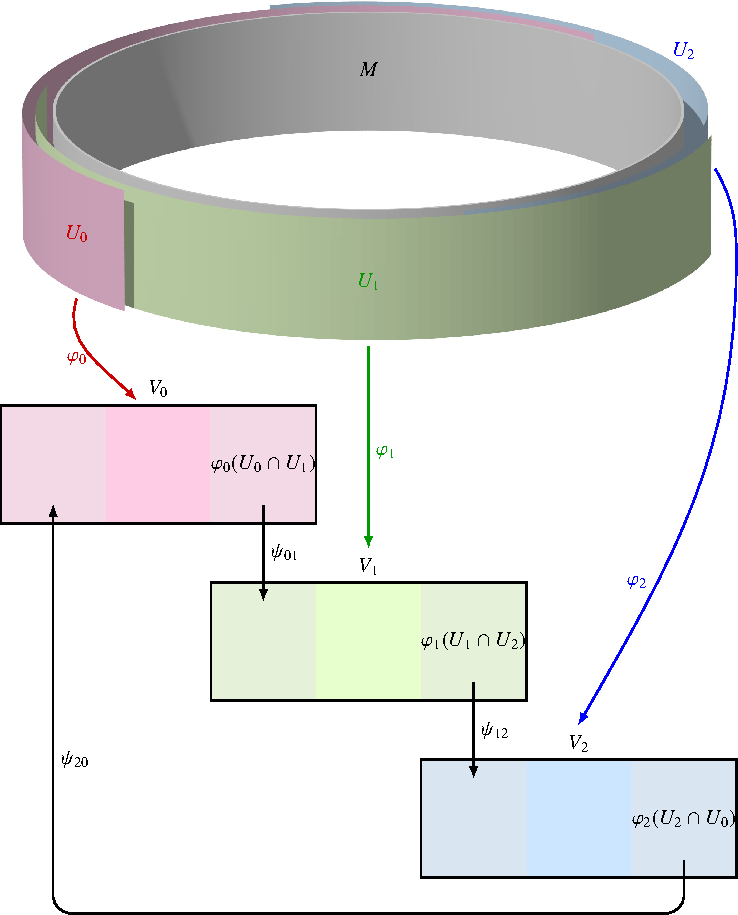
\includegraphics{chapters/040-green/images/band.pdf}
\caption{Zylindrisches Band mit drei Karten und drei Kartenwechselgebieten,
in denen die Determinante der Ableitung des Kartenwechsels positiv ist.
Das Band ist daher orientierbar.
\label{buch:green:green:fig:band}}
\end{figure}

Die Mannigfaltigkeit $M$ von Abbildung~\ref{buch:green:green:fig:band}
wird durch die drei Kartengebiete
\begin{align*}
V_0&=\psi_0(U_0) = \biggl(-\frac{\pi}3,\frac{5\pi}3\biggr)\times(-l,l),
\\
V_1&=\psi_1(U_1) = \biggl(-\frac{\pi}3,\frac{5\pi}3\biggr)\times(-l,l)
\\
\text{und}\qquad
V_2&=\psi_2(U_2) = \biggl(-\frac{\pi}3,\frac{5\pi}3\biggr)\times(-l,l)
\end{align*}
und die Kartenwechselabbildungen
\begin{align*}
\psi_{01}&\colon
\psi_0(U_0\cap U_1)
\to
V_1
:(x,y) \mapsto \biggl(x-\frac{2\pi}3,y\biggr)
\\
\psi_{12}&\colon
\psi_1(U_1\cap U_2)
\to
V_2
:(x,y) \mapsto \biggl(x-\frac{2\pi}3,y\biggr)
\\
\psi_{20}&\colon
\psi_2(U_2\cap U_0)
\to
V_0
:(x,y) \mapsto \biggl(x-\frac{2\pi}3,y\biggr)
\end{align*}
Die drei Kartengebiete sind Rechtecke.
Die Ableitung der Kartenwechselabbildung hat als Matrix die Einheitsmatrix,
die positive Determinante hat.
Auf dieser Mannigfaltigkeit gibt es eine 2-Form, die in jedem 
Kartengebiet durch $dx\wedge dy$ gegeben ist.
Insbesondere hat diese 2-Form keine Nullstellen.
\end{beispiel}


\begin{beispiel}
\label{buch:green:green:beispiel:moebius}
%
% fig-moebius.tex
%
% (c) 2025 Prof Dr Andreas Müller
%
\begin{figure}
\centering
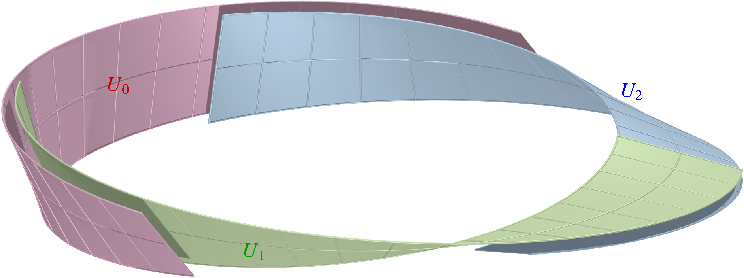
\includegraphics{chapters/040-green/images/moebius.pdf}
\caption{Durch Änderung einer einzigen Kartenwechselabbildung entsteht
ein Atlas für ein Möbius-Band, welches nicht orientierbar ist.
\label{buch:green:green:fig:moebius}}
\end{figure}
%
Durch Änderung der Kartenwechselabbildung in
\begin{align*}
\psi_{12}&\colon
\psi_1(U_1\cap U_2)
\to
V_2
:(x,y) \mapsto \biggl(x-\frac{2\pi}3,-y\biggr)
\end{align*}
entsteht ein neuer Atlas, der aber nicht mehr ein zylindrisches Band
beschreibt.
In Abbildung~\ref{buch:green:green:fig:moebius} wird das gemeinsame
Gebiet $U_1\cap U_2$ der grünen und der blauen Karte gespiegelt,
was einem um $180^\circ$ verdrehten Band entspricht.
Dies ein Möbius-Band.

Auf dem Möbius-Band gibt es keine 2-Form ohne Nullstellen.
\index{Mobius-Band@Möbius-Band}%
Gäbe es eine solche 2-Form $\omega$, dann könnten wir die Komponenten
in der roten und der grünen Karte $U_0$ und $U_1$ so ändern, dass
$\omega$ auf beiden durch $dx\wedge dy$ gegeben ist.
Dann ist nur noch eine Darstellung $u(x,y)\,dx\wedge dy$ für die 
blaue Karte $U_2$ gefunden werden.
Auf dem Überschneidungsgebiet $\varphi_2(U_0\cap U_2)$ muss $u(x,y)=1$
sein.
Auf dem Überschneidungsgebiet $\varphi_2(U_1\cap U_2)$ ist die 
Determinante des Kartenwechsels $-1$, d.~h.~dort muss $u(x,y)=-1$
sein.
$u(x,y)$ ist daher eine differenzierbare Funktion auf dem zusammenhängend
Rechteck $V_2$, welche am einen Ende den Wert $1$ und am anderen den 
Wert $-1$ haben muss.
Nach dem Zwischenwertsatz muss diese Funktion eine Nullstelle haben.
\end{beispiel}

Der Unterschied zwischen den beiden Mannigfaltigkeiten der Beispiele
\ref{buch:green:green:beispiel:band}
und
\ref{buch:green:green:beispiel:moebius}
ist, dass das Möbius-Band nicht orientierbar ist.
Lässt man eine Ameise entlang dem Möbius-Band krabbeln, wird sie
sich nach einem Umlauf um das Band auf der anderen Seite des Bandes
wiederfinden.
Sie muss also nochmals einen weiteren Umlauf ausführen, um wieder
am Ausgangspunkt auf der gleichen Seite wie beim Start anzukommen.

\begin{definition}
Eine differenzierbare zweidimensionale Mannigfaltigkeit heisst 
\emph{orientierbar}, wenn es eine 2-Form gibt, die nirgends
\index{orientierbar}%
verschwindet.
\end{definition}

Die Konstruktion des Atlas in den Beispielen zeigt, dass es eine
alternative Beschreibung einer orientierbaren Mannigfaltigkeit.
Für die orientierbare Mannigfaltigkeit wurde ein Atlas gefunden,
dessen Kartenwechsel alle positive Determinanten hatten.
Für das nicht orientierbare Möbius-Band war dies nicht möglich.

\begin{definition}[orientierbarer Atlas]
Ein \emph{orientierbarer Atlas} einer differenzierbaren Mannigfaltigkeit
\index{Atlas!orientierbar}%
ist ein Atlas, dessen Kartenwechsel alle positive Determinante haben.
\index{Kartenwechsel}%
\end{definition}

Man kann zeigen, dass diese beiden Definitionen sind.
Dies ist der Inhalt des folgenden Satzes, den wir aber nicht
beweisen werden.

\begin{satz}
Eine zweidimensionale Mannigfaltigkeit ist genau dann orientierbar,
wenn es einen orientierbaren Atlas gibt.
\end{satz}



%
% Der Satz von Green
%
\section{Der Satz von Green
\label{buch:green:section:green}}
\kopfrechts{Der Satz von Green}
Der Hauptsatz der Infinitesimalrechnung besagt, dass man das Integral
\index{Hauptsatz der Infinitesimalrechnung}%
einer Ableitung aus den Werten am Intervallende erhalten kann.
Diese Idee wurde bereits in Kapitel~\ref{chapter:kurvenintegral} auf
das Integral einer 1-Form verallgemeinert.
Das Integral eines Differentials $df$ entlang einer Kurve ist durch
die Werte der Funktion $f$ in den Endpunkten gegeben.
Im vorliegenden Abschnitt soll eine ähnliche Ausssage für Integrale
von 2-Formen über zweidimensionale Gebiete abgeleitet werden.
Der Satz von Green stellt einen Zusammenhang zwischen dem Integral
gewisser Ableitungen über das Innere eines Gebietes und den Werten
auf dem Rand dar.
Es soll gezeigt werden, dass die Ableitung eine natürlich Erweiterung
des Differentials $df$ einer Funktion ist.
In späteren Kapiteln soll dies dann zum allgemeinen Satz von Stokes
verallgemeinert werden.
\index{Satz!von Stokes}%
Die auf diese Weise aus dem Differential $d$ erhaltenen
Differentialoperatoren sind die natürlichen Operatoren, die für
eine koordinatenfreie Formulierung von Naturgesetzen geeignet sind.
So wie wir das Differential bereits als Gradient einer Funktion
interpretiert haben, soll die Ableitung von 1- und 2-Formen später
als die in den Anwendungen weit verbreitet Operation der Rotation
und der Divergenz erkannt werden.

%
% Zerlegung in Koordinatengebiete
%
\subsection{Zerlegung in Koordinatengebiete
\label{buch:green:satzvongreen:subsection:zerlegung}}
In Abschnitt~\ref{buch:kurvenintegral:section:zerlegung} wurde gezeigt,
wie sich ein Integral einer $1$-Form über eine Kurve mit Hilfe einer
Zerlegung der Einheit durch endlich viele beliebig oft differenzierbare
Funktionen $g_i$ in eine endlich Summe
\[
\int_{\gamma} \alpha = \sum_i \int_{\gamma} g_i\alpha_i
\]
von Integralen von differenzierbaren 1-Formen zerlegen, wobei der
Träger von $g_i$ immer in einem Koordinatengebiet enthalten war.
Diese Vorgehensweise lässt sich auch auf zweidimensionale Gebiete
übertragen.

Im folgenden betrachten wir nur kompakte Mannigfaltigketen, da nicht
kompakte Mannigfaltigkeiten ohnehin zu nicht definierten Integralen
führen können.

Ein Quader in $\mathbb{R}^n$ ist ein kartesisches Produkt
\[
Q
=
(a_1,b_1)
\times\dots\times
(a_n,b_n)
=
\{
(x^1,\dots,x^n)\in\mathbb{R}^n
\mid
a_i < x^i < b_i
\;\forall i=1,\dots,n
\}.
\]
Die Funktionen
\[
g_Q(x)
=
g_{a_1,b_1}(x^1)\dots g_{a_n,b_n}(x^n)
\]
sind beliebig oft differenzierbare Funktionen, die genau im Quader
$Q$ von $0$ verschieden sind.

Eine beschränkte offene Menge $U\subset\mathbb{R}^n$ kann, wie in
%
% fig-quader.tex
%
% (c) 2025 Prof Dr Andreas Müller
%
\begin{figure}
\centering
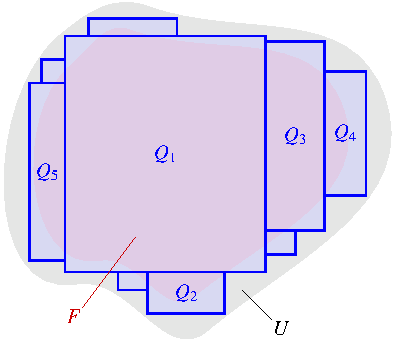
\includegraphics{chapters/040-green/images/quader.pdf}
\caption{Äpproximation einer offenen Menge $U$ durch Quader $Q_i$,
die ihrerseits den Träger $F$ einer Funktion vollständig überdecken.
\label{buch:green:fig:quader}}
\end{figure}
%
Abbildung~\ref{buch:green:fig:quader} am zweidimensionalen Beispiel gezeigt,
von innen durch Quader approximiert werden.
Ist $F\subset U$ eine abgeschlossene Teilmenge, dann ist sie auch
kompakt und kann daher von endlich vielen Quadern überdeckt werden.
Durch Addition der zugehörigen Funktionen der Form $g_Q$ kann man also
eine beliebig oft differenzierbare Funktion finden, die auf $F$ von
$0$ verschieden ist und deren Träger ganz in $U$ enthalten ist.

Wir wenden diese Überlegung jetzt auf die Kartengebiete eines
Atlas $(U_\alpha)_{\alpha\in I}$ einer kompakten Mannigfaltigkeit an.
Da die Mannigfaltigkeit kompakt ist, dürfen wir sogar annehmen, dass
der Atlas aus nur endlich vielen Karten besteht.
In jedem Kartengebiet wählen wir jetzt eine Vereinigung $V_\alpha$
von offenen Quadern so, dass auch die Mengen $V_\alpha$ die ganze
Mannigfaltigkeit überdecken.

\begin{satz}
Sei $(U_\alpha,\varphi_\alpha)$ eine endliche Familie von Karten,
die eine kompakte Mannigfaltigkeit überdecken.
Dann gibt es Teilmengen $V_\alpha\subset U_\alpha$, die endliche
Vereingungen von Quadern sind derart, dass die eingeschränkten Karten
$(V_\alpha,\varphi_\alpha\mathstrut_{|V_\alpha})$ ebenfalls einen Atlas
bilden.
\end{satz}

\begin{proof}
Zu jedem $\alpha$ und Punkt $x\in U_\alpha$ gibt es einen offenen
Quader $Q_{x,\alpha}$, der $x$ enthält und in $U_\alpha$ enthalten
ist: $x\in Q_{x,\alpha}\subset U_\alpha$.
Die Vereinigung der $Q_{x,\alpha}$ ist eine Überdeckung der
Mannigfaltigkeit.
Da die Mannigfaltigkeit $M$ kompakt ist, gibt es auch eine endliche 
Teilmenge, die bereits $M$ überdeckt.
Bildet man für jedes $\alpha$ die Mengen $V_\alpha$ aus den Quadern
$Q_{x,\alpha}$, dann ist $V_\alpha$ eine Überdeckung der Mannigfaltigkeit
der verlangten Art.
\end{proof}

In einer Überdeckung einer Mannigfaltigkeit durch die Vereinigungen
$V_\alpha$ von Quadern kann man eine Menge von beliebig oft
differenzierbaren Funktionen
$g_\alpha$ ableiten, die genau auf $V_\alpha$ von $0$ verschieden
sind.
Da die $V_\alpha$ eine Überdeckung bilden, ist die Summe
\[
G(x) = \sum_{\alpha} g_\alpha(x)
\]
auf der ganzen Mannigfaltigkeit von $0$ verschieden und kann dazu
benutzt werden, die Funktionen $g_\alpha$ auf
\[
h_\alpha(x) = \frac{1}{G(x)}\,g_\alpha(x)
\]
zu normieren, die eine Zerlegung der Einheit bilden.

Auf einem Kartengebiet einer zweidimensionalen Mannigfaltigkeit
ist bereits bekannt, wie eine 2-Form integriert werden kann.
Mit einer Zerlegung der Einheit, wie sie oben konstruiert worden ist,
lässt sich jetzt das Integral einer beliebigen 2-Form jetzt über
die ganze Mannigfaltigkeit erstrecken.
Dazu schreibt man
\[
\int_M \alpha
=
\int_M \sum_{\alpha}h_\alpha\,\alpha
=
\int_{V_\alpha} h_\alpha\,\alpha.
\]
Dies ist möglich, weil $h_\alpha\,\alpha$ nur innerhalb von $V_\alpha$
von $0$ verschieden ist.
Die 2-Form $h_\alpha\,\alpha$ kann im Kartengebiet durch die
Komponenten dargestellt und integriert werden.

%
% Interal in einem Koordinatengebiet
%
\subsection{Integral in einem Koordinatengebiet}
Dank der Zerlegung eines Integrals gemäss
Abschnitt~\ref{buch:green:satzvongreen:subsection:zerlegung}
muss in diesem Abschnitt nur noch das Integral einer 2-Form in
einem Koordinatengebiet berechnet werden.
Wir nehmen daher an, dass die 2-Form durch
\[
\omega
=
a_{ik}(x)\,dx^i\wedge dx^k
\]
gegeben ist, wobei die Koeffizienten $a_{ik}(x)$ ausserhalb
von $V_\alpha$ verschwindet.

%
% Integral über ein Gebiet ohne Rand
%
\subsubsection{Integral über ein Gebiet ohne Rand}
In den Koordinaten der Karte wird das Integral der 2-Form $\omega$
durch
\begin{equation}
\int_M \omega
=
\int_{\varphi_\alpha(V_\alpha)}
a_{ik}(x)\, v(x)
\,dx^1\,dx^2
\label{buch:green:green:eqn:koordinatenform}
\end{equation}
gegeben.
% XXX was ist v(x)
Da $\omega$ ausserhalb von $V_\alpha$ verschwindet, können wir $\omega$
durch 0 auf ganz $\mathbb{R}^2$ ausdehnen und integrieren.

Für das im Satz von Green angestrebte Resultat berechnen wird das
Integral einer 2-Form der Form
\[
\frac{\partial f_i}{\partial x^k}(x)\, dx^i \wedge dx^k,
\]
wobei $i\ne k$ ist.
Einsetzen der Definition in
\eqref{buch:green:green:eqn:koordinatenform}
ergibt das Integral
\begin{align*}
\int_M\omega
&=
\int\hspace*{-2mm}\int_{\varphi_\alpha(V_\alpha)}
\frac{\partial f_i}{\partial x^k}(x)
\, dx^i \, dx^k.
\intertext{Nach dem Satz von Fubini können die Integrale über die
Variablen unabhängig voneinander durchgeführt werden.
Wir schreiben daher}
&=
\int_{-\infty}^{\infty}
\int_{-\infty}^{\infty}
\frac{\partial f_i}{\partial x^k}(x)
\,dx^k
\,dx^i.
\intertext{Das innere Integral kann ausgeführt werden und ergibt}
&=
\int_{-\infty}^{\infty}
\biggl[f_i(x)\biggr]_{-\infty}^{\infty}
\,dx^i.
\intertext{Da $f_i(x)$ ausserhalb des Gebietes $\varphi_\alpha(V_\alpha)$
verschwindet, ist der Integrand $0$ und damit auch}
\int_{V_\alpha} \omega
&=
0.
\end{align*}
Für eine 2-Form, deren Koeffizienten eine Ableitung sind, verschwindet
also das Integral über ein Gebiet ohne Rand.

%
% Der Rand eines Gebietes
%
\subsubsection{Der Rand eines Gebietes}
%
% fig-randkarten.tex
%
% (c) 2025 Prof Dr Andreas Müller
%
\begin{figure}
\centering
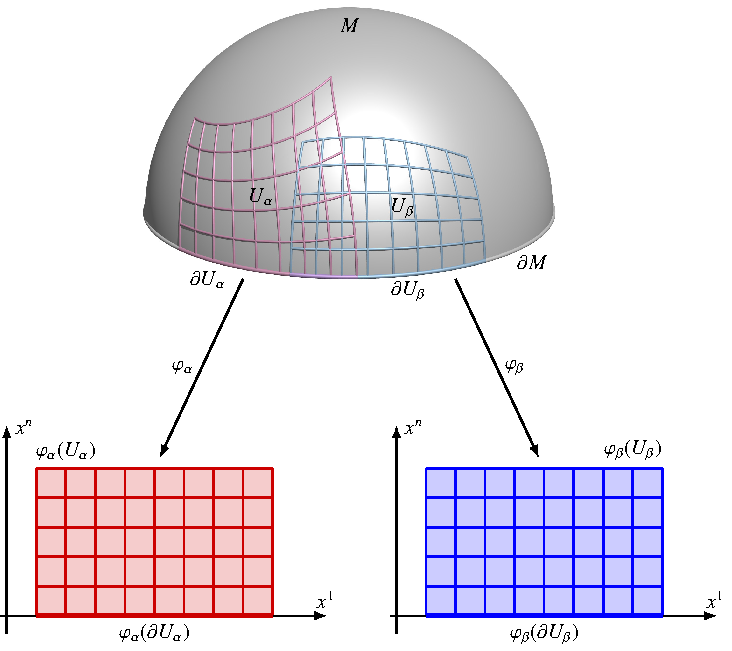
\includegraphics{chapters/040-green/images/randkarten.pdf}
\caption{Eine Mannigfaltigkeit mit Rand hat Karten, die eine offene
Teilmenge von $\{x^n=0\}$ als Rand enthalten.
Kartenwechsel sind beliebig oft differenzierbare Abbildungen, die
Randteile in Randteile abbilden (ausgezogene Linien entlang der
Hyperebene $\{x^n=0\}$).
\label{buch:green:green:fig:randkarten}}
\end{figure}

Der Wert des Kurvenintegrals der 1-Form $df$ entlang einer
Kurve zwischen zwei Punkten $A$ und $B$ in einer $n$-dimensionalen
Mannigfaltigkeit wird durch die Werte von $f$ in den Endpunkten
gegeben.
Das Integrationsgebiet $[a,b]$ ist nicht eine eindimensionale
Mannigfaltigkeit, da in einer solchen jeder Punkt eine Umgebung
hat, die homöomorph zu einem offenen Intervall in $\mathbb{R}$ ist.
Die beiden Endpunkt haben diese Eigenschaft nicht, sie haben eine
Umgebung, die homöomorph zum halboffenen Intervall $[0,1)$ für
den Anfangspunkt und $(-1,0]$ für den Endpunkt sind.
Man sagt, $[a,b]$ sei eine eindimensionale Mannigfaltigkeit mit
Rand.
\index{Rand}%

Eine $n$-dimensionale differenzierbare Mannigfaltigkeit kann
ähnlich dadurch definiert werden, dass zusätzliche Arten von
Karten zugelassen werden.
Eine Karte $(U,\varphi)$ von $M$ ist eine Abbildung
$\varphi \colon U\to\mathbb{R}^n$, die ein Homöomorphismus
zwischen $U$ und einer offenen Teilmenge von
\[
\{
(x^1,\dots,x^n) \in\mathbb{R}^n
\mid
x^n\ge 0
\}
\]
ist.
$U$ kann also wie bisher eine offene Menge sein oder sie kann 
einen Teil der Hyperebene $x^n=0$ enthalten.
Dieser Teil $\partial U=\varphi^{-1}(\{x^n = 0\})$ ist ein Randstück und
durch weglassen der letzten Koordinate bekommen wir eine Kartenabbildung
$\varphi_{|\partial U}\colon \partial U \to \mathbb{R}^{n-1}$ für das
Randstück.
Für die Kartenwechsel wird verlangt, dass sie und die Ableitungen
beliebig oft differenzierbar sind, dass aber auch die Kartenwechsel
auf den Randteilen umkehrbare differenzierbare Abbildungen zwischen
offenen Mengen von $\mathbb{R}^{n-1}$ sein müssen.
Die Kartengebiete mit Rand müssen also einen Atlas für den Rand
der differenzierbaren Mannigfaltigkeit ergeben.

%
% Integral über den Rand
%
\subsubsection{Integral über den Rand}
%
% fig-greenrand2d.tex
%
% (c) 2025 Prof Dr Andreas Müller
%
\begin{figure}
\centering
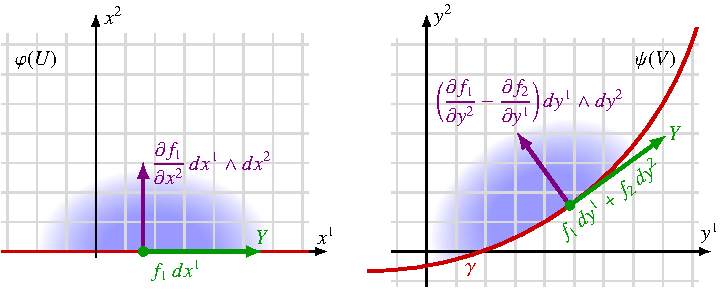
\includegraphics{chapters/040-green/images/greenrand2d.pdf}
\caption{Berechnung des Integrals einer 2-Form über ein Gebiet mit Rand.
Falls der Rand die Achse $x^2=0$ ist, ist das Integral im Wesentlichen
eine Stammfunktion des Koeffizienten.
Für gekrümmten Rand setzt sich das Integral aus den Komponenten der
Normalen zusammen.
\label{buch:green:green:fig:greenrand2d}}
\end{figure}
%
Der Satz von Green, der weiter unten formuliert wird, stellt einen
Zusammenhang eines Integrals einer 2-Form über das Gebiet und eines
Integrals einer 1-Form über den Rand her.
\index{Randintegral}%
Dieser Zusammenhang ist in Abbildung~\ref{buch:green:green:fig:greenrand2d}
links dargestellt.
Das Integral der 
\[
\omega = \frac{\partial f_1}{\partial x_2}\,dx^1\wedge dx^2
\]
über das Kartengebiet $U$ der Karte $(U,\varphi)$ ist das Integral 
von $\omega$ gegeben durch
\begin{align*}
\int_{\varphi(U)} \omega
&=
\int_{-\infty}^{\infty}
\biggl(
\int_{0}^{\infty}
\frac{\partial f_1}{\partial x^2}(x^1,x^2)\,dx^2
\biggr)\,dx^1.
\intertext{Das $x^2$-Integral kann sofort ausgeführt werden und ist}
&=
\int_{-\infty}^{\infty}
\bigl[ f_1(x^1,x^2) \bigr]_{0}^{\infty}
\,dx^1
=
-
\int_{-\infty}^\infty
f_1(x^1,0)
\,dx^1.
\end{align*}
Das letzte Integral ist das Integral der 1-Form $f_1\,dx^1$ entlang
der $x^1$-Achse, die den Rand bildet.

Dieses Argument ist auch anwendbar, wenn der Rand gekrümmt ist,
wie dies in Abbildung~\ref{buch:green:green:fig:greenrand}
unten dargestellt ist.
%
% fig-greenrand.tex
%
% (c) 2025 Prof Dr Andreas Müller
%
\begin{figure}
\centering
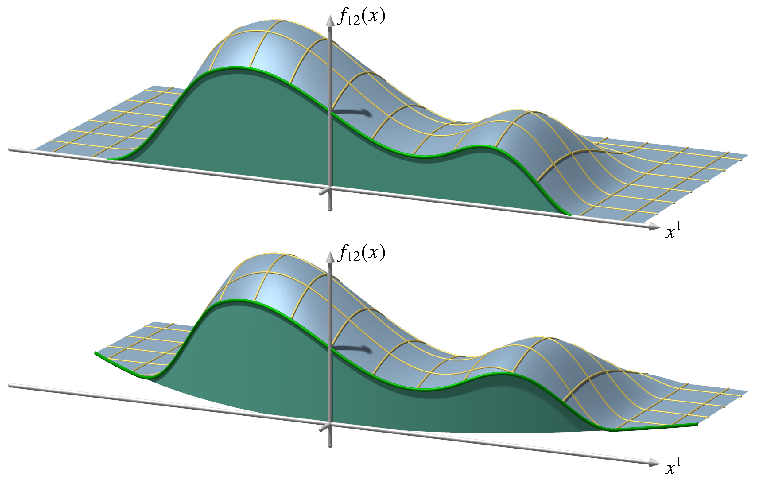
\includegraphics{chapters/040-green/images/greenrand.pdf}
\caption{Berechnung des Beitrags zum Integral einer 2-Form
$\omega = f_{12}(x)\,dx^1\wedge dx^2$, die am Rand nicht
verschwindet.
\label{buch:green:green:fig:greenrand}}
\end{figure}
%
Ist $g$ eine Funktion so, dass der Graph $x^2=g(x^1)$ den Rand
beschreibt, dann kann man das Integrationsgebiet mit den Koordinaten
\[
(y^1,y^2)
=
(x^1,x^2-g(x^1))
\]
beschreiben.
In den $(y^1,y^2)$-Koordinaten bekommt das Gebiet damit einen geraden
Rand.

Der Koordinatenwechsel für die 1-Formen ist
\begin{align*}
dy^1 &= dx^1 \\
dy^2 &= dx^2 - g'(x^1)\,dx^1.
\end{align*}
Für die daraus gebildete 2-Form gilt
\[
dy^1\wedge dy^2
=
dx^1 \wedge (dx^2 - g'(x^1)\,dx^1)
=
dx^1\wedge dx^2
-
g'(x^1)\,\underbrace{dx^1\wedge dx^1}_{\displaystyle=0}
=
dx^1\wedge dx^2.
\]

Die zu integrierende 2-Form ist
\[
\omega
=
\frac{\partial f_1}{\partial x^2}(x^1,x^2)
\,dx^1\wedge dx^2
=
\frac{\partial f_1}{\partial x^2}(y^1,y^2+g(y^1)).
\,dy^1\wedge dy^2
\]
Das Hinzufügen des nicht von $x^2$ abhängigen Terms $g(y^1)$ ändert
nichts an der Ableitung.
Das Integral der 2-Form $\omega$ wird dann
\begin{align*}
\int \omega
&=
\int_{-\infty}^{\infty}
\int_{g(x^1)}^\infty
\frac{\partial f_1}{\partial x^2}
\,dx^2
\,dx^1.
\intertext{Die Grenzen des $x^1$ Integrals sind durch den Rand des
Gebiets vorgegeben und sind im Moment nicht wichtig, da sie in den
$(y^1,y^2)$-Koordinaten ohnehin wegfallen.
Das Integral wird in $(y^1,y^2)$-Koordinaten zu}
&=
\int_{\dots}^{\dots}
\int_0^\infty
\frac{\partial f_1}{\partial x^2}(y^1,y^2+g(y^1))
\,dy^2
\,dy^1
\\
&=
\int_{-\infty}^\infty
\bigl[
f_1(y^1,y^2+g(y^1))
\bigr]_{0}^\infty
\,dy^1
\\
&=
-
\int_{-\infty}^\infty
f_1(y^1,g(y^1))
\,dy^1.
\intertext{Das letzte Integral ist das Integral der 1-Form $f_1\,dy^1$
entlang der Randkurve $\gamma(t) = (t,g(t))$:}
&=
- \int_\gamma f_1(\gamma(t))\,dt.
\end{align*}
Auch für einen gekrümmten Rand kann man also das Integral der 2-Form,
die eine Ableitung enthält, über das Gebiet durch ein Integral
einer 1-Form über den Rand ausdrücken.

%
% Integral einer 2-Form in einer Karte mit Rand
%
\subsubsection{Integral einer 2-Form in einer Karte mit Rand}
Sei jetzt $V_\alpha$ ein Randkartengebiet einer 2-dimensionalen
Mannigfaltigkeit mit Rand.
Wieder betrachten wir eine 2-Form $\omega$ genz spezieller Form,
in diesem Fall die Form
\[
\omega
=
\biggl(
\frac{\partial f_2}{\partial y^1}
-
\frac{\partial f_1}{\partial y^2}
\biggr)
\,
dy^1\wedge dy^2.
\]
Abbildung~\ref{buch:green:green:fig:greenrand2d} rechts zeigt diese
Situation.
Wir betrachten die beiden Summanden unabhängig voneinander.
Nach der Berechnung des vorangegangenen Abschnitts wird das Integral
des ersten Summanden
\begin{align*}
\int_{\psi(V)}
\frac{\partial f_1}{\partial y^2}\,dy^1\wedge dy^2
&=
-\int_{\gamma} f_1\,dy^1.
\intertext{Für den zweiten Term können wir das gleiche Argument
angeben, allerdings zeigt die Abbildung, dass das Integral nur bis
zur roten Kurve $\gamma$ erstreckt wird, während es beim ersten Summanden
bei der roten Kurve begann.
Dieser Term bekommt daher ein anderes Vorzeichen.
Wir erhalten}
\frac{\partial f_2}{\partial y^1}\,dy^1\wedge dy^2
&=
\int_{\gamma} f_2\,dy^2.
\end{align*}
Zusammen ergibt sich
\[
\int_{\psi(V)}
\biggl(
\frac{\partial f_1}{\partial y^2}
-
\frac{\partial f_2}{\partial y^1}
\biggr)\, dy^1\wedge dy^2
=
-
\int_\gamma 
\bigl(
f_1\,dy^1
+
f_2\,dy^2
\bigr).
\]
Indem wir das Vorzeichen kehren, folgt die Formel
\begin{equation}
\int_{\psi(V)}
\biggl(
\frac{\partial f_2}{\partial y^1}
-
\frac{\partial f_1}{\partial y^2}
\biggr)\, dy^1\wedge dy^2
=
\int_{\gamma}
\bigl(
f_1\,dy^1
+
f_2\,dy^2
\bigr).
\label{buch:green:green:eqn:integralmitrand}
\end{equation}
Sie stellt einen Zusammenhang her zwischen einer 1-Form auf dem 
Rand und Ableitungen im Inneren des Gebietes.

%
% Die äussere Ableitung einer 1-Form
%
\subsection{Die äussere Ableitung einer 1-Form}
Der Integrand des linken Integrals in
\eqref{buch:green:green:eqn:integralmitrand}
hat offenbar eine besondere Bedeutung, die die folgende Definition
rechtfertigt.

\begin{definition}[äussere Ableitung in $\Omega^2(\mathbb{R}^2)$]
\label{buch:green:green:definition:aeussereableitung2d}
Die {\em äussere Ableitung} der in Komponenten gegebenen 1-Form
\[
\alpha = f_1(x)\,dx^1 + f_2(x)\,dx^2
\]
ist
\[
d\alpha
=
\frac{\partial f_2}{\partial x^1}(x)
\,dx^1\wedge dx^2
+
\frac{\partial f_1}{\partial x^2}(x)
\,dx^2\wedge dx^1
=
\biggl(
\frac{\partial f_2}{\partial x^1}(x)
-
\frac{\partial f_1}{\partial x^2}(x)
\biggr)
\,dx^1\wedge dx^2.
\]
\end{definition}

Die Definition könnte ad hoc erscheinen, um eine Abkürzung für den
Integranden~\eqref{buch:green:green:eqn:integralmitrand} zu erhalten.
Warum treten nur die Ableitungen von $f_1$ nach $x^2$ und
$f_2$ nach $x^1$ auf?
Die folgende, allgemeinere Definition der äusseren Ableitung 
einer beliebigen 1-Form auf einer Mannigfaltigkeit beliebiger 
Dimension, liefert eine Erklärung.

\begin{definition}[äussere Ableitung in $\Omega^2(M)$]
Die {\em äussere Ableitung} einer 1-Form $\alpha\in\Omega^1(M)$ ist
\index{aussere Ableitung@äussere Ableitung}
in einer Karte, in der die 1-Form durch die Komponentendarstellung
\[
\alpha
=
f_1(x)\,dx^1 + \dots + f_n(x)\, dx^n
=
\sum_{i=1}^n f_i(x)\,dx^i
\]
gegeben ist,
definiert durch die Komponenten
\[
d\alpha
=
\sum_{k=1}^n
\frac{\partial f_i}{\partial x^k}(x)
\,dx^k\wedge dx^i.
\]
\end{definition}

Die Terme mit $i=k$ enthalten die 2-Form $dx^k\wedge dx^i=dx^k\wedge dx^k=0$
verschwinden in der Summe.
Im Spezialfall $n=2$ entsteht daher
\begin{align*}
d\alpha
&=
\frac{\partial f_1}{\partial x^1}\,\underbrace{dx^1\wedge dx^1}_{\displaystyle=0}
+
\frac{\partial f_1}{\partial x^2}\,\underbrace{dx^2\wedge dx^1}_{\displaystyle-dx^1\wedge dx^2}
+
\frac{\partial f_2}{\partial x^1}\,dx^1\wedge dx^2
+
\frac{\partial f_2}{\partial x^2}\,\underbrace{dx^2\wedge dx^2}_{\displaystyle=0}
\\
&=
\biggl(
\frac{\partial f_2}{\partial x^1}
-
\frac{\partial f_1}{\partial x^2}
\biggr)
\,dx^1\wedge dx^2.
\end{align*}
Dies stimmt mit der
Definition~\ref{buch:green:green:definition:aeussereableitung2d}
überein.

%
% Der Satz von Green
%
\subsection{Der Satz von Green}
Wenn das ganze Definitionsgebiet mit einer einzigen Karbte beschrieben
werden kann, lässt sich aus den Rechnungen der vorangegangenen
Abschnitten der folgende Satz von Green ableiten.
\index{Satz!von Green}%
Wir nehmen dazu an, dass der Rand des Gebietes $U$ wie in
Abbildung~\ref{buch:green:green:fig:greenbeweis}
durch Funktionen $y_-(x)$ und $y_+(x)$ für den unter und oberen Rand
bzw.~durch Funktionen $x_-(y)$ und $x_+(y)$ für den linken und rechten
Rand möglich ist.
Die Randkurve selbst lässt sich dann sowohl durch die $x$-Koordinate
als
\[
x\mapsto (x,y_-(x)) 
\qquad\text{bzw.}\qquad
x\mapsto (x,y_+(x)) 
\]
als auch durch die $y$-Koordinate als
\[
y\mapsto (x_-(y),y) 
\qquad\text{bzw.}\qquad
y\mapsto (x_+(y),y) 
\]
parametrisieren.
%
% fig-greenbeweis.tex
%
% (c) 2025 Prof Dr Andreas Müller
%
\begin{figure}
\centering
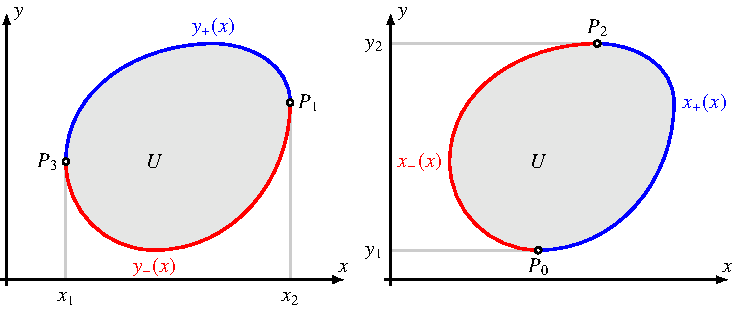
\includegraphics{chapters/040-green/images/greenbeweis.pdf}
\caption{Parametrisierung des Randes des Gebietes $U$ für den
Beweis des klassischen Satzes von Green.
\label{buch:green:green:fig:greenbeweis}}
\end{figure}
%

\begin{satz}[Green]
Für zwei Funktionen $f(x,y)$ und $f(x,y)$ auf einem Gebiet
$U\subset\mathbb{R}^2$ mit Randkurve $\gamma$, die das Gebiet
im Gegenuhrzeigersinn umlaufen.
Dann gilt
\begin{align*}
\underset{U}{\int\!\!\!\int}
\frac{\partial g}{\partial x}(x,y)
-
\frac{\partial f}{\partial y}(x,y)
\,dx\,dy
&=
\int_{x_1}^{x^2}
\int_{y_-(x)}^{y_+(x)}
\frac{\partial g}{\partial x}(x,y)
-
\frac{\partial f}{\partial y}(x,y)
\,dy
\,dx
\\
&=
\int_{y_1}^{y_2}
\int_{x_-(y)}^{x_+(y)}
\frac{\partial g}{\partial x}(x,y)
-
\frac{\partial f}{\partial y}(x,y)
\,dx
\,dy
\\
=
\oint_\gamma f(x,y)\,dx + g(x,y)\,dy
&=
\int_a^b f(\gamma(t))\,\dot{x}(t) + g(\gamma(t))\,\dot{y}(t)\,dt.
\end{align*}
\end{satz}

\begin{proof}
Die beiden Terme des Integranden werden unabhängig voneinander
unter Verwendung der verschiedenen Randparametrisierungen
berechnet.
Die Reihenfolge der Integrationen über $x$ bzw.~$y$ kann daher
in den beiden Teilintegralen vertauscht werden:
\begin{align}
I_f
=
\int_{x_1}^{x_2}
\int_{y_-(x)}^{y_+(x)}
\frac{\partial f}{\partial y}(x,y)
\,dy
\,dx
&=
\int_{x_1}^{x_2}
\bigl[
f(x,y)
\bigr]_{y_-(x)}^{y_+(x)}
\,dx
\notag
\\
&=
\int_{x_1}^{x_2}
f(x,y_+(x))
-
f(x,y_-(x))
\,dx
\label{buch:green:green:proof:eqn:xparam}
\\
I_g
=
\int_{y_1}^{y_2}
\int_{x_-(y)}^{x_+(y)}
\frac{\partial g}{\partial x}(x,y)
\,dx
\,dy
&=
\int_{y_1}^{y_2}
\bigl[
g(x,y)
\bigr]_{x_-(y)}^{x_+(y)}
\,dy
\notag
\\
&=
\int_{y_1}^{y_2}
g(x_+(y),y)
-
g(x_-(y),y)
\,dy.
\label{buch:green:green:proof:eqn:yparam}
\end{align}
Zusammen ist das Doppelintegral $-I_f+I_g$.
Dieses Integral lässt sich jetzt nach 
\eqref{buch:green:green:proof:eqn:xparam}
und
\eqref{buch:green:green:proof:eqn:yparam}
durch Randintegrale berechnen:
\begin{align*}
-I_f+I_g
&=
\int_{x_1}^{x_2}
f(x,y_-(x))
\,dx
+
\int_{y_1}^{y^2}
g(x_+(y),y)
\,dy
\\
&\qquad
+
\int_{x_2}^{x_1}
f(x,y_+(x))
\,dx
+
\int_{y_2}^{y_1}
g(x_-(y),y)
\,dy.
\intertext{Das Integral lässt sich aufteilen in Integrale, die sich
alle mit dem Parameter $x$ schreiben lassen.
Damit dies möglich wird, müssen wir es in vier Teile}
&=
\phantom{+}
%\int_{x_+(y_1)}^{x_2}
\int_{P_0}^{P_1}
f(x,y_-(x))
+
g(x,y_-(x))\,y_-'(x)\,dx
\\
&\phantom{=}
+
%\int_{x_2}^{x_+(y_2)}
\int_{P_1}^{P_2}
f(x,y_+(x))
+
g(x,y_+(x))\,y_+(x)\, dx
\\
&\phantom{=}
+
%\int_{x_-(y_2)}^{x_1}
\int_{P_2}^{P_3}
f(x,y_+(x))
+
g(x,y_+(x))\,y_+'(x)\,dx
\\
&\phantom{=}
+
%\int_{x_1}^{x_-(y_1)}
\int_{P_3}^{P_0}
f(x,y_-(x))
+
g(x,y_-(x))\, y_-'(x) \,dx
\intertext{zwischen den hervorgehobenen Punkten
$P_0=(x_-(y_1),y_1)$, $P_1=(x_2,y_+(x_2))$, $P_2=(x_+(y_2),y_2)$ und
$P_3=(x_1,y_+(x_1))$
zerlegen.
In allen vier Integralen hat der Integrand die gleiche Form.
In einer beliebigen Parametrisierung
$\gamma\colon [a,b]\to\mathbb{R}^2: t\mapsto(x(t),y(t))$
der Randkurve wird das Integral
zu}
&=
\int_a^b
f(x(t),y(t))\,\dot{x}(t) 
+
g(x(t),y(t))\,\dot{y}(t) 
\,dt
\\
&=
\oint_\gamma f(x,y)\,dx + g(x,y)\,dy.
\end{align*}
Damit ist der Satz von Green bewiesen.
\end{proof}

%
% Der Satz von Green als Spezialfall des Satzes von Stokes
%
\subsection{Der Satz von Green als Spezialfall des Satzes von Stokes}
Die Motivation für den Satz von Green war der Zusammenhang zwischen
dem Integral einer 2-Form auf einer zweidimensionalen Mannigfaltigkeit
mit Rand und dem Integral einer 1-Form.
Dieser Satz gilt aber nicht nur auf einer 2-dimensionalen Mannigfaltigkeit,
sondern kann für beliebige 2-dimensionale Mannigfaltigkeiten, die in
eine $n$-dimensionale Mannigfaltigkeit eingebettet sind.
\index{Satz!von Stokes}%

\begin{satz}[Stokes]
\label{buch:green:green:satz:stokes}
Sie $\alpha$ eine 1-Form auf der $n$-dimensionalen Mannigfaltigkeit $M$.
Sie $S$ eine zweidimensionale Mannigfaltigkeit mit Rand und
$f\colon S\to M$ eine differenzierbare Einbettung von $S$ in $M$.
Dann ist $f^*\alpha$ eine differenzierbare 1-Form auf $S$ und
$df^*\alpha=f^*d\alpha$.
Schreibt man $\omega=f^*\alpha$,
dann gilt
\[
\int_S d\omega
=
\int_{\partial S}\omega.
\]
\end{satz}

Der Satz von Green ist der Spezialfall $M=\mathbb{R}^2$ und $S=U$.


%
% Geschlossene 1-Formen und Wegunabhängigkeit
%
\section{Geschlossene 1-Formen und Wegunabhängigkeit
\label{buch:green:section:geschlossen}}
Für die 1-Formen $df$ ist die Berechnung des Wegintegrals besonders
einfach, da $f$ als ``Stammfunktion'' betrachtet werden kann.
Nicht jede 1-Form lässt sich als Differential einer Funktion $df$ 
schreiben.
In diesem Abschnitt soll ein Kriterium dafür gefunden werden, 
ob eine 1-Form $\alpha$ als $\alpha=df$ geschrieben werden kann.

%
% Äusseres Differential von $df$
%
\subsection{Äusseres Differential von $df$}
Ist $f$ eine Funktion auf der Mannigfaltigkeit $M$, dann können wir
die 1-Form $\alpha = df$ bilden.
In einer Karte ist $\alpha$ durch die partiellen Ableitungen
\[
\alpha
=
\sum_{i=1}^n
\frac{\partial f}{\partial x^i}(x)\,dx^i
\]
gegeben.
Für die äussere Ableitung von $df$, bildet man
\[
d\alpha
=
\sum_{i,k=1}^n
\frac{\partial}{\partial x^k}
\frac{\partial f}{\partial x^i}(x)\,
dx^k
\wedge
dx^i.
\]
Die Terme mit $i=k$ sind Vielfache von $dx^i\wedge dx^i=0$, tragen
also nichts bei.
In der Summe (man beachte die einsteinsche Summenkonvention)
tritt jedes Paar von verschiedenen Indizes genau zweimal in verschiedener
Reihenfolge auf, wegen $dx^i\wedge dx^k = - dx^k \wedge dx^i$ kann man
\begin{align}
d\alpha
&=
\sum_{i < k}
\biggl(
\frac{\partial^2 f}{\partial x^i\,\partial x^k}(x)\, dx^i\wedge dx^k
+
\frac{\partial^2 f}{\partial x^k\,\partial x^i}(x)\, dx^k\wedge dx^i
\biggr)
\notag
\\
&=
\sum_{i < k}
\biggl(
\frac{\partial^2 f}{\partial x^i\,\partial x^k}(x)
-
\frac{\partial^2 f}{\partial x^k\,\partial x^i}(x)
\biggr)
\, dx^i\wedge dx^k
\label{buch:green:geschlossen:eqn:dalpha}
\end{align}
schreiben.
Da $f$ beliebig oft stetig differenzierbar sind, sind die partiellen
Ableitungen vertauschbar, der Klammerausdruck in
\eqref{buch:green:geschlossen:eqn:dalpha}
verschwindet und es folgt $d\alpha = 0$.

\begin{definition}[Geschlossene 1-Form]
\index{geschlossene 1-Form}%
Eine 1-Form $\alpha$ heisst {\em geschlossen}, wenn ihr äusseres
Differential $d\alpha=0$ verschwindet.
\end{definition}

Es liegt nahe zu vermuten, dass jede geschlossene 1-Form als Differential
geschrieben werden kann.
Dies ist jedoch nicht richtig, wie das folgende Beispiel zeigt.

\begin{beispiel}
\label{buch:green:geschlossen:beispiel:wegabhaengig}
Wir betrachten die 1-Form
\[
\alpha
=
\frac{-y}{x^2+y^2}\,dx
+
\frac{x}{x^2+y^2}\,dy
\]
auf $M=\mathbb{R}^2\setminus\{0\}$.
Die äussere Ableitung ist
\begin{align*}
d\alpha
&=
\frac{\partial}{\partial y}
\frac{-y}{x^2+y^2}
\,dy\wedge dx
+
\frac{\partial}{\partial x}
\frac{x}{x^2+y^2}
\,dx\wedge dy
\\
&=
\biggl(
\frac{\partial}{\partial y}
\frac{y}{x^2+y^2}
+
\frac{\partial}{\partial x}
\frac{x}{x^2+y^2}
\biggr)
\,dx\wedge dy.
\intertext{Die beiden Ableitungen gehen durch Vertauschen von $x$ und $y$
ineinander über.
Sie können leicht mit Maxima oder einem anderen Computeralgebraprogramm
berechnet werden und sind}
&=
\biggl(
\frac{x^2-y^2}{(x^2+y^2)^2}
+
\frac{y^2-x^2}{(x^2+y^2)^2}
\biggr)
\,dx\wedge dy
=
0,
\end{align*}
$\alpha$ ist also eine geschlossene 1-Form.

Allerdings lässt sich $\alpha$ nicht als Differential schreiben.
Dann liessen sich nämlich die Wegintegrale für die Halbkreise
\begin{align*}
\gamma_+&\colon [0,\pi] \to \mathbb{R}^2 : t \mapsto (\cos t,\sin t)
\\
\gamma_-&\colon [0,\pi] \to \mathbb{R}^2 : t \mapsto (\cos t,-\sin t)
\end{align*}
von $(1,0)$ nach $(-1,0)$ in der oberen bzw.~der unteren Halbebene
einfach als Differenz der Funktionswerte berechnen, sie müssten
also gleich sein.
% XXX Graphik für die Definition der Wege \gamma_+ und \gamma_-
Wir berechnen daher die beiden Wegintegrale:
\begin{align*}
\int_{\gamma_+}\alpha
&=
\int_{0}^{\pi}
\frac{-\sin t}{\cos^2 t+\sin^2t}(-\sin t)
+
\frac{\cos t}{\cos^2 t+\sin^2t}\cos t
\,dt
\\
&=
\int_0^\pi \sin^2 t+\cos^2 t\,dt
=
\int_0^\pi 
\,dt
=
\pi,
\\
\int_{\gamma_-}\alpha
&=
\int_{0}^{\pi}
\frac{-(-\sin t)}{\cos^2 t+\sin^2t}(-\sin t)
+
\frac{\cos t}{\cos^2 t+\sin^2t}(-\cos t)
\,dt
\\
&=
-\int_0^\pi \sin^2 t+\cos^2 t\,dt
=
-\int_0^\pi 
\,dt
=
-\pi.
\end{align*}
Da die beiden Wegintegrale verschieden sind, kann $\alpha$ kein
Differential sein.
\end{beispiel}

%
% Wegunabhängigkeit
%
\subsection{Wegunabhängigkeit}
Das Beispiel \ref{buch:green:geschlossen:beispiel:wegabhaengig}
verrät auch, warum die Vermutung falsch ist.
Wenn $\alpha=df$ ist, dann liefert jeder Weg zwischen zwei Punkten
$A$ und $B$ den gleichen Wert $f(B)-f(A)$ des Wegintegrals von $\alpha$.
Tatsächlich geben im Beispiel Wege auf verschiedenen Seiten des Nullpunktes
verschiedene Werte des Wegintegrals.
Die Vermutung kann also nur stimmen, wenn diese Situation ausgeschlossen
werden kann.

\begin{definition}[Einfach zusammenhängend]
Eine Mannigfaltigkeit heisst {\em einfach zusammenhängend}, wenn sich
\index{einfach zusammenhangend@einfach zusammenhängend}
jeder geschlossene Weg differenzierbar in einen Punkt zusammenziehen
lässt.
\end{definition}

Eine Mannigfaltigkeit ist insbesondere einfach zusammenhängend, wenn
die ganze Mannigfaltigkeit in einen Punkt zusammenziehbar ist.
%
% fig-homotopie.tex
%
% (c) 2025 Prof Dr Andreas Müller
%
\begin{figure}
\centering
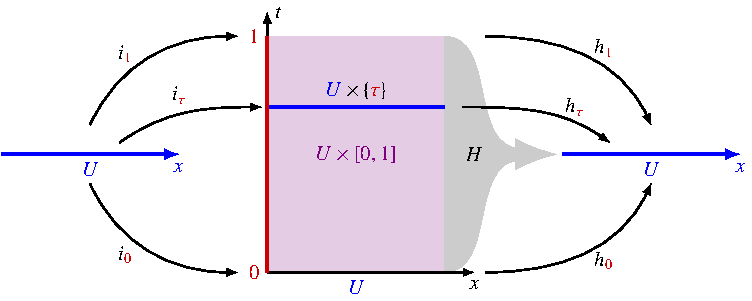
\includegraphics{chapters/060-pformen/images/homotopie.pdf}
\caption{Eine Homotopie $H$ ist eine Abbildung $U\times[0,1]$, die
die Abbildung $h_0\colon U\to U$ in die Abbildung $h_1\colon U\to U$
deformiert.
Die Abbildung $h_{\tau}$ entsteht durch Einsetzen des Wertes $\tau$
in das zweite Argument von $H$, was gleichbedeutend ist mit der
Zusammensetzung von $H$ mit $i_\tau$: $h_\tau=H\circ i_\tau$.
\label{buch:pformen:fig:homotopie}}
\end{figure}
%
Die Abbildung
\[
H
\colon
\mathbb{R}^n\times [0,1]
:
(x,t) \mapsto H_t(x) = (1-t)x
\]
deformiert die identische Abbildung
\(
H_0(x)
=
x
\)
in die Nullabbildung
\(
H_1(x) = 0
\).
Indem man den Parameter $t$ von $0$ auf $1$ anwachsen lässt, werden
alle Punkte in den Nullpunkte gezogen.
Ein geschlossener Weg $\gamma(s)$ wird dabei differenzierbar in
den konstanten geschlossenen Weg $H_1(\gamma(s))=0$ zusammengezogen.
Ein Abbildung dieser Art heisst eine {\em Homotopie}
\index{Homotopie}%
der identischen Abbildung in die Nullabbildung.

\begin{definition}[differenzierbare Homotopie]
Eine differenzierbare Homotopie zweier Wege $\gamma_0$ und $\gamma_1$
in der differenzierbaren Manigfaltigkeit mit den gleichen Endpunkten
ist eine differenzierbare Abbildung
\[
H
\colon
[0,1]\times[0,1]
\to
M
\]
mit
\[
\left.
\begin{aligned}
H_0(s) &= \gamma_0(s)\\
H_1(s) &= \gamma_1(s)
\end{aligned}
\;
\right\}
\qquad\text{und}\qquad
\left\{\;
\begin{aligned}
H_t(0) &= \gamma_0(0) = \gamma_1(0) = A\\
H_t(1) &= \gamma_0(1) = \gamma_1(1) = B.
\end{aligned}
\right.
\]
Wege, die durch eine differenzierbare Homotopie verbunden sind,
heissen {\em homotop} (Abbildung~\ref{buch:green:fig:homotopie}).
\end{definition}

Die Kugeloberfläche $S^2$ ist einfach zusammenhängend, zum Beispiel
kann man den Äquator im Nullpunkt zusammenzieht.
Es gibt aber im Gegensatz zum Beispiel $\mathbb{R}^n$ keine Homotopie
der identischen Abbildung der Kugeloberfläche in eine konstante
Abbildung.

\begin{satz}
\label{buch:green:geschlossen:satz:wegunabhaengig}
Für eine geschlossene 1-Form $\alpha$ ist das Integral
\[
\int_{\gamma_0}\alpha = \int_{\gamma_1} \alpha
\]
über zwei homotope Wege $\gamma_0$ und $\gamma_1$ gleich.
\end{satz}

\begin{proof}
Wir betrachten die Homotopie $H:[0,1]\times[0,1]\to M$ zwischen
den beiden Wegen.
Dann ist nach dem Satz von Green
\[
\int_{[0,1]\times[0,1]}
TH^*(d\alpha)
=
\int_{\partial [0,1]^2} TH^*(\alpha).
\]
Wegen $d\alpha=0$ verschwindet das Integral auf der linken Seite.
Das Integral auf der rechten Seite setzt sich aus vier Wegintegralen
zusammen, einem für jede Kante des Quadrates $\partial[0,1]^2$.
Das Integral entlang der Seite $[0,1]\times\{0\}$ ergibt das Integral
entlang dem $H_0(s) = \gamma_0(s)$.
Die Kante $[0,1]\times\{1\}$ ergibt das Integral entlang der
Kurve $H_1(s) = \gamma_1(s)$, allerdings wird der Weg in umgekehrter
Richtung durchlaufen.
Die beiden Kanten $\{0\}\times[0,1]$ und $\{1\}\times[0,1]$ sind
konstant, das Integral entlang dieser Kanten ist daher $0$.
Von den Wegintegralen bleiben daher
\[
0
=
\int_{\partial[0,1]^2} (TH)^*(\alpha)
=
\int_{\gamma_0} \alpha
-
\int_{\gamma_1} \alpha
\quad\Rightarrow\quad
\int_{\gamma_0} \alpha
=
\int_{\gamma_1} \alpha.
\]
Die beiden Wegintegrale sind gleich.
\end{proof}

Im Beispiel~\ref{buch:green:geschlossen:beispiel:wegabhaengig}
war zwar $d\alpha=0$ aber es gab keine Homotpie, die die Wege
entlang dem Einheitskreis vom Punkt $(1,0)$ zum Punkt $(-1,0)$
in der oberen bzw.~der unteren Halbebene verbindet.

%
% Geschlossene 1-Formen auf einfach zusammenhängenden Gebieten
%
\subsection{Geschlossene 1-Formen auf einfach zusammenhängenden Gebieten}
Die Wegunabhängigkeit des Wegintegrals für eine geschlossene 1-Form
kann jetzt verwendet werden, um eine Funktion $f$ zu finden, deren
Differential die gegebene 1-Form ist.

\begin{satz}
\label{buch:green:geschlossen:satz:poincare}
Eine geschlossene 1-Form $\alpha$ auf einem einfach zusammenhängenden
Gebiet kann als $\alpha=df$ geschrieben werden.
\end{satz}

Die nach Satz~\ref{buch:green:geschlossen:satz:poincare}
existierende Funktion $f$ ist nicht eindeutig, denn mit $f$ hat
auch $f+c$ für jede Konstante $c\in\mathbb{R}$ das Differential
\[
d(f+c) = df + dc = df = \alpha.
\]
Der Beweis wird klar machen, was die Bedeutung

\begin{proof}
Sie $\alpha$ eine geschlossene 1-Form auf der einfach zusammenhängenden
Mannigfaltigkeit $M$.
Ausserdem wird ein Punkt $A\in M$ gewählt.
Für jeden Punkt $P\in M$ wählen wir einen Weg $\gamma:\colon[0,1]\to M$,
der $A$ mit $P$ verbindet.
Die Funktion $f\colon M\to\mathbb{R}$ wird als
\[
f(P) = \int_{\gamma} \alpha.
\]
Nach Satz~\ref{buch:green:geschlossen:satz:wegunabhaengig} ist das eine
konsistente Definition, denn jede Wahl des Weges ergibt den gleichen
Wert des Integrals.
Wir müssen nachprüfen, dass $df=\alpha$ ist.

Um die Ableitung zu berechnen, verwenden wir eine Karte, in der sich die
1-Form als
\[
\alpha = a_i(x)\, dx^i
\]
schreiben lässt.
Wir müssen zeigen, dass
\[
a_i(x) = \frac{\partial f}{\partial x^i}(x)
\]
ist.
Dazu verwenden wir nochmals die Möglichkeit, den Weg $\gamma$ frei wählen
zu können.
Wir wählen in so, dass $\gamma(1)=x$ ist und
\[
\dot{\gamma}(1) = e_i
\]
der Standardbasisvektor ist.
Nach Definition der Funktion $f$ ist
\[
\frac{d}{dt}
f(\gamma(t))
\biggl|_{t=1}
=
\langle
\alpha,
e_i
\rangle
=
a_i(x).
\]
Da dies für jede andere Koordinate auch gilt, folgt $df=\alpha$.
\end{proof}

Im Beweis wurde stillschweigend angenommen, dass sich für jedes
Paar von Punkten in der Mannigfaltigkeit ein Weg finden lässt, der
die beiden Punkte verbindet.
Nicht jede Mannigfaltigkeit hat diese Eigenschaft.
Die Oberflächen der Planeten des Sonnensystems sind zweidimensionale
Mannigfaltigkeiten $S^2$, auf jeder einzelnen sind Punkte untereinander
verbindbar.
Es gibt aber keine Wege zwischen den einzelnen Planeten.
Man nennt eine Mannigfaltigkeit {\em wegzusammenhängend}, wenn es zu jedem
Paar von Punkten einen verbindenden Weg gibt.

Der Beweis ist also nur korrekt für wegzusammenhängende Mannigfaltigkeiten.
Trotzdem gilt der Satz allgemein.
Dazu beginnt man mit einem Punkt $A_0\in M$ und berechnet die Funktion $f$
für jeden Punkt $P\in M$ der sich mit $A_0$ verbinden lässt.
Damit ist $f$ auf der sogenannten {\em Wegzusammenhangskomponente} von $A_0$
definiert.
Die Zusammenhangskomponente ist eine Untermannigfaltigkeit von $M$.
Falls sie nicht ganz $M$ umfasst, wählen wir einen weiteren Punkt $A_1$,
der nicht mit $A_0$ verbunden werden kann, und definieren $f$ auf der
Wegzusammenhangskomponente von $A_1$.
Auf diese Weise lässt sich die Funktion in jeder Wegzusammenhangskomponente
definieren.

Eine andere Wahl des Starpunktes $A_k$ in jeder Wegzusammenhangskomponente
verändert die Werte der Funktion $f$ in der Zusammenhangskomponente
um eine Konstante $c_k$.
Die Funktion $f$ ist daher nur bis auf eine Konstante $c_k\in\mathbb{R}$
in jeder Zusammenhangskomponente definiert.

%
% Potentialfelder
%
\subsection{Potentialfelder}
Das Gravitationsfeld ist bekannt dafür, dass die Arbeit, die gegen
das Feld geleistet werden muss, um einen Massepunkt von einem Punkt $A$
zu einem Punkt $B$ zu bewegen, nicht von der Wahl des Weges abhängt.
Die Unabhängigkeit vom Weg garantiert, dass es
eine Funktion $U(x)$ gibt, mit der man den Energieunterschied
$U(B)-U(A)$ berechnen kann.
Die Funktion $U$ heisst das Potential.
In der Physik wird es meistens noch durch die Masse geteilt,
diese Unterscheidung ist für die aktuelle Diskussion jedoch unwichtig.

Sei $\gamma(t)$ die Kurve, auf der sich der Massepunkt 
bewegt.
Die Leistung gegen das Gravitationsfeld ist dann
$\langle dU, \dot{g}(t)\rangle$.
Die Funktion $U$ kann als Wegintegral von $dU$ rekonstruiert werden.

\begin{definition}[Potential]
Eine 1-Form $\omega$ heisst ein {\em Potentialfeld}, wenn es eine
Funktion $U$ gibt derart, dass $dU=\omega$.
\end{definition}

Nach Satz~\ref{buch:green:geschlossen:satz:poincare} ist $\omega$
auf einem einfach zusammenhängenden Gebiet genau dann ein Potentialfeld,
wenn $d\omega=0$ ist.

\begin{beispiel}
Für das Gravitationsfeld einer Masse $M$ im Nullpunkt des Koordinatensystems
ist die potentielle Energie
\[
U(x,y,z)
=
-\frac{GM}{r}.
\]
Die äussere Ableitung 
\begin{align*}
dU
&=
\frac{\partial U}{\partial x}\,dx
+
\frac{\partial U}{\partial y}\,dy
+
\frac{\partial U}{\partial z}\,dz
\\
&=
-\frac{GM}{r^3}\bigl(
x\,dx
+
y\,dy
+
z\,dz
\bigr)
\end{align*}
Im nächsten Kapitel wird gezeigt, dass die Funktion $U$ noch eine
weitere Eigenschaft hat, nämlich dass die Divergenz verschwindet.
Daraus wird sich dann die Gleichung $\Delta U=0$ ergeben.
\end{beispiel}



\uebungsabschnitt

\aufgabetoplevel{chapters/040-green/uebungsaufgaben}
\begin{uebungsaufgaben}
\uebungsaufgabe{401}
\end{uebungsaufgaben}
\enduebungsabschnitt

